\chapter{Podstawy teoretyczne}\label{chap:podstawy}

W rozdziale omówiono trzy obszary wiedzy stanowiące podstawę teoretyczną dla
dalszej części pracy: ewolucję systemów agentowych, mechanizmy generowania
wspomaganego wyszukiwaniem oraz specyfikę dokumentów prawnych ze szczególnym
uwzględnieniem polskich dokumentów ubezpieczeniowych jako środowiska
ewaluacyjnego.

\section{Systemy agentowe}\label{sec:systemy-agentowe}

Systemy oparte na dużych modelach językowych przeszły ewolucję od potoków
przetwarzających proste zapytania do autonomicznych systemów realizujących
złożone cele. Kolejne podrozdziały porządkują tę dziedzinę -- punktem wyjścia
jest definicja agenta, po której następuje przegląd wariantów
architektonicznych, od układów pojedynczych po złożone topologie rozproszone.

\subsection{Pojęcie agenta}\label{subsec:pojecie-agenta}

Pojęcie agenta pochodzi z~wczesnych badań nad sztuczną inteligencją i~wyprzedza
powstanie dużych modeli językowych. Wooldridge i~Jennings określili go jako byt
obliczeniowy osadzony w~środowisku, który potrafi realizować założone cele bez
nadzoru. Definicja ta zakłada cztery główne cechy: autonomię, zdolność
społeczną, reaktywność i~proaktywność~\cite{wooldridge1995intelligent}. System
operuje bez ciągłej ingerencji operatora, komunikuje się z~innymi podmiotami,
reaguje na zmiany otoczenia i~inicjuje działania celowe. Kryteria te,
sformułowane pierwotnie z~myślą o~systemach robotycznych i~symulacjach
wieloagentowych, pozostają aktualne w~kontekście współczesnych agentów
językowych -- zmianie podlega tylko środowisko, które nie jest już przestrzenią
fizyczną, lecz cyfrową: interfejsy programistyczne, repozytoria dokumentów,
bazy wiedzy.

Wang i~in. wyodrębnili cztery współpracujące elementy agenta: profil, pamięć,
planowanie oraz działanie~\cite{wang2024survey}. Profil nadaje systemowi
konkretną rolę operacyjną i~ustala cele nadrzędne. Pamięć zachowuje zebrane
informacje między kolejnymi krokami. Planowanie dzieli złożony problem na
wykonalne etapy. Moduł działania zamienia wynik rozumowania na operacje
techniczne, takie jak odpytanie bazy danych lub wywołanie zewnętrznego skryptu.
Podział ten wymusza zaprojektowanie niezależnych komponentów -- różnice między
poszczególnymi architekturami agentowymi wynikają z~decyzji podjętych w~tych
czterech obszarach.

Integracja modelu z~narzędziami nie gwarantuje jego pełnej autonomii, co
podkreślają Xi i~in.~\cite{xi2025rise}. System wyposażony w~dostęp do sieci
może działać wyłącznie jako reaktywny generator tekstu. Warunkiem autonomii
jest umiejętność podtrzymywania celu, monitorowania postępów oraz korygowania
strategii w~razie wystąpienia błędu. Wiele istniejących rozwiązań stanowią
modele z~dostępem do zewnętrznych interfejsów, niespełniające kryteriów
proaktywności i~działania zorientowanego na cel.

Pętla decyzyjna stanowi fundament działania agenta. Agent odbiera bieżący stan
środowiska, interpretuje go za pomocą modelu językowego i~wybiera kolejny krok
-- na przykład wywołanie narzędzia. Po wykonaniu akcji obserwuje jej wynik
i~aktualizuje stan zadania. Pętla powtarza się aż do zakończenia
zadania~\cite{yao2022react}. Architektury agentowe różnią się sposobem
organizacji pętli decyzyjnej, liczbą jej iteracji oraz podziałem zadań między
agentów~\cite{wang2024survey, xi2025rise}. Schemat blokowy przedstawiony na
rysunku~\ref{fig:petla-decyzyjna} ilustruje fazy pojedynczego cyklu
decyzyjnego.

\begin{figure}[H]
  \caption{Pętla decyzyjna agenta}\label{fig:petla-decyzyjna}
  \centering
  \begin{adjustbox}{max width=0.82\textwidth}
    \begin{tikzpicture}[
        node distance=0.7cm and 1.2cm,
        state/.style={rectangle, draw, rounded corners=4pt,
            minimum width=2.6cm, minimum height=0.9cm,
            align=center, font=\small,
            fill=violet!8, draw=violet!50},
        tool/.style={rectangle, draw, rounded corners=4pt,
            minimum width=2.6cm, minimum height=0.9cm,
            align=center, font=\small,
            fill=gray!7, draw=gray!40},
        arrow/.style={->, >=stealth, draw=gray!60},
        label/.style={font=\footnotesize\itshape, text=gray!55!black}
      ]
      \node[state] (obs)  {Obserwacja\\stanu};
      \node[state, right=2.2cm of obs]  (llm)  {Model\\językowy};
      \node[state, right=2.2cm of llm]  (dec)  {Decyzja\\o~działaniu};
      \node[tool,  below=1.4cm of dec]  (tool) {Wywołanie\\narzędzia};
      \node[state, left=2.2cm  of tool] (upd)  {Aktualizacja\\stanu zadania};
      \draw[arrow] (obs)  -- node[above, label]{percepcja}    (llm);
      \draw[arrow] (llm)  -- node[above, label]{wnioskowanie} (dec);
      \draw[arrow] (dec)  -- node[right, label]{akcja}        (tool);
      \draw[arrow] (tool) -- node[below, label]{wynik}        (upd);
      \draw[arrow] (upd)  -- node[below, label]{nowa obserwacja}
      (obs |- upd) -- (obs);
    \end{tikzpicture}
  \end{adjustbox}
  \zrodlo{opracowanie własne}
\end{figure}

Funkcjonowanie agenta warunkują trzy elementy: instrukcja systemowa
(ang.~\textit{system prompt}), okno kontekstowe (ang.~\textit{context window})
i~schemat narzędzi. Instrukcja systemowa określa rolę agenta, ograniczenia
i~format wyjścia. Okno kontekstowe pełni rolę pamięci roboczej -- gromadzi
historię dialogu, wyniki narzędzi, pobrane dowody i~pośrednie kroki
rozumowania. Schemat narzędzi opisuje, jakie operacje agent może wywołać
i~w~jaki sposób. Niejasna instrukcja systemowa, zbyt małe okno kontekstowe oraz
niepełny opis narzędzi stanowią główne przyczyny błędów w~implementacji
architektur agentowych~\cite{wang2024survey, schick2023toolformer}.

\subsection{Klasyfikacja architektur agentowych}\label{subsec:klasyfikacja-architektur-agentowych}

Architektury agentowe klasyfikuje się według różnych kryteriów. Dwa najczęściej
stosowane podziały dotyczą liczby agentów uczestniczących w~realizacji zadania
oraz stopnia autonomii systemu podczas podejmowania
decyzji~\cite{wang2024survey, xi2025rise, guo2024large}. Kryteria te są
ortogonalne -- system jednoagentowy może być w~pełni autonomiczny, a~system
wieloagentowy może działać według ściśle deterministycznego 
schematu~\cite{weng2023agent}.

Najprostszym wariantem jest architektura jednoagentowa, w~której pojedynczy
model językowy samodzielnie obsługuje cały cykl: interpretuje zapytanie,
wywołuje narzędzia i~formułuje odpowiedź. Zaletą tego podejścia jest prostota
implementacji i~przewidywalność zachowania -- każdy krok jest realizowany przez
ten sam model z~tym samym oknem kontekstowym. Wadą jest natomiast ograniczona
zdolność do równoległego przetwarzania oraz trudność w~obsłudze zadań
wymagających jednoczesnej specjalizacji w~wielu
dziedzinach~\cite{wang2024survey}. W~praktyce architektury jednoagentowe są
odpowiednie dla zadań o~dobrze zdefiniowanym zakresie, takich jak odpowiadanie
na pytania na podstawie zamkniętego korpusu dokumentów.

Architektury wieloagentowe dzielą zadanie między kilka współpracujących
instancji modelu, z~których każda pełni odrębną rolę -- planisty, wykonawcy,
weryfikatora lub specjalisty dziedzinowego~\cite{guo2024large}. Podział ten
pozwala na równoległe przetwarzanie niezależnych podzadań i~ogranicza ryzyko
przeciążenia pojedynczego okna kontekstowego. Złożoność ta skutkuje jednak
większą liczbą wywołań modelu, wyższym zużyciem tokenów oraz trudniejszą
diagnostyką błędów, ponieważ awaria dowolnego węzła utrudnia lokalizację
przyczyny niepowodzenia~\cite{guo2024large, xi2025rise}.

Niezależnie od liczby agentów, architektury różnią się również stopniem
autonomii w~podejmowaniu decyzji~\cite{weng2023agentm wang2024survey, xi2025rise}. Wyróżnia
się układy deterministyczne, realizujące z~góry zdefiniowaną sekwencję kroków,
oraz układy w~pełni autonomiczne, w~których agent samodzielnie planuje
i~modyfikuje działania na podstawie uzyskanych wyników. Przykładem pierwszego
podejścia jest klasyczny potok RAG, drugiego -- architektura ReAct, w~której
model werbalizuje tok rozumowania i~wywołuje narzędzia, definiując przebieg
zadania~\cite{yao2022react}. W~praktyce powszechnie stosowane są podejścia
hybrydowe: deterministyczny szkielet orkiestracji ogranicza przestrzeń
decyzyjną, a~model dobiera argumenty narzędzi i~interpretuje wyniki.

Rysunek~\ref{fig:podzial-architektur-agentowych} przedstawia klasyfikację
omawianych topologii według dwóch głównych kryteriów. Gałąź lewa obejmuje
układy jednoagentowe -- od modelu sterowanego wyłącznie instrukcją systemową,
przez architekturę ReAct z~iteracyjnym rozumowaniem, po układ planer--wykonawca
z~jawnym etapem planowania. Gałąź prawa grupuje architektury wieloagentowe
według dominującego wzorca przepływu informacji: potokowego, hierarchicznego,
tablicowego i~opartego na routingu. Węzeł \textit{Model z~instrukcją systemową}
pełni rolę punktu odniesienia.

\begin{figure}[H]
  \caption{Podział architektur agentowych}\label{fig:podzial-architektur-agentowych}
  \centering
  \begin{adjustbox}{max width=\textwidth}
    \begin{tikzpicture}[
        every node/.style={font=\scriptsize},
        branch/.style={rectangle, draw, rounded corners=3pt,
            minimum width=2.0cm, minimum height=0.7cm, align=center},
        leaf/.style={rectangle, draw, rounded corners=3pt,
            minimum width=2.0cm, minimum height=0.9cm,
            text width=1.9cm, align=center},
        arrow/.style={->, >=stealth, thin, draw=gray!60},
        root/.style={rectangle, draw, rounded corners=4pt,
            minimum width=2.6cm, minimum height=0.8cm, align=center,
            fill=gray!7, draw=gray!40, font=\scriptsize\bfseries}
      ]
      \node[root] (root) at (0,0) {Architektury agentowe\\LLM};

      \node[branch, fill=violet!8, draw=violet!40]
      (single) at (-4.2,-1.6) {Jednoagentowe};
      \node[branch, fill=teal!7, draw=teal!40]
      (multi)  at (5.1,-1.6)  {Wieloagentowe};

      \draw[arrow] (root.south) -- ++(0,-0.3) -| (single.north);
      \draw[arrow] (root.south) -- ++(0,-0.3) -| (multi.north);

      \node[leaf, fill=violet!5, draw=violet!30]
      (llm)   at (-6.8,-3.5) {Model\\z~instrukcją\\systemową};
      \node[leaf, fill=violet!5, draw=violet!30]
      (react) at (-4.2,-3.5) {ReAct};
      \node[leaf, fill=violet!5, draw=violet!30]
      (ps)    at (-1.6,-3.5) {Planer--\\wykonawca};

      \draw[arrow] (single.south) -- ++(0,-0.2) -| (llm.north);
      \draw[arrow] (single.south) -- ++(0,-0.2) -| (react.north);
      \draw[arrow] (single.south) -- ++(0,-0.2) -| (ps.north);

      \foreach \x/\txt in {-6.8/brak iteracji, -4.2/iteracja, -1.6/planowanie}{
          \node[draw=gray!25, fill=gray!4, rounded corners=2pt,
            font=\tiny\itshape, text=gray!55!black, inner sep=2pt]
          at (\x,-4.55) {\txt};
        }

      \node[leaf, fill=teal!5, draw=teal!30]
      (seq)  at (1.2,-3.5) {Deterministyczna};
      \node[leaf, fill=teal!5, draw=teal!30]
      (hier) at (3.8,-3.5) {Hierarchiczna};
      \node[leaf, fill=teal!5, draw=teal!30]
      (tab)  at (6.4,-3.5) {Tablicowa};
      \node[leaf, fill=teal!5, draw=teal!30]
      (rout) at (9.0,-3.5) {Router--\\specjalista};

      \draw[arrow] (multi.south) -- ++(0,-0.2) -| (seq.north);
      \draw[arrow] (multi.south) -- ++(0,-0.2) -| (hier.north);
      \draw[arrow] (multi.south) -- ++(0,-0.2) -| (tab.north);
      \draw[arrow] (multi.south) -- ++(0,-0.2) -| (rout.north);

      \foreach \x/\txt in {1.2/potok, 3.8/delegacja, 6.4/współpraca, 9.0/routing}{
          \node[draw=gray!25, fill=gray!4, rounded corners=2pt,
            font=\tiny\itshape, text=gray!55!black, inner sep=2pt]
          at (\x,-4.55) {\txt};
        }
    \end{tikzpicture}
  \end{adjustbox}
  \zrodlo{opracowanie własne na podstawie literatury}
\end{figure}

\subsection{Architektury jednoagentowe}\label{subsec:architektury-jednoagentowe}

Najprostszą architekturą jednoagentową jest model sterowany wyłącznie
instrukcją systemową, który odpowiada na podstawie wiedzy odwzorowanej w~wagach
modelu podczas trenowania. Taki wariant stanowi naturalny punkt odniesienia
(ang.~\textit{baseline}), ponieważ pozwala oddzielić wpływ użycia narzędzi,
wyszukiwania i~sterowania od samej jakości modelu bazowego. Sprawdza się przy
pytaniach, których odpowiedź została odwzorowana w~parametrach modelu, ale
wykazuje trudności przy pytaniach wymagających danych aktualnych lub ściśle
dziedzinowych -- skutkuje to generowaniem nieprawdziwych informacji,
określanych jako halucynacje~\cite{ji2023survey}. Ograniczenie to jest
szczególnie istotne w~dziedzinach takich jak prawo czy ubezpieczenia, gdzie
precyzja i~aktualność informacji mają bezpośrednie znaczenie dla użytkownika.

Jedną z~propozycji rozwiązania tego problemu jest topologia ReAct, która włącza
do procesu decyzyjnego ślad rozumowania (ang.~\textit{reasoning trace}). Agent
naprzemiennie werbalizuje plany, wykonuje akcję i~przetwarza jej rezultat,
a~decyzja o~kolejnym kroku opiera się na pozyskanych dowodach, a~nie na z~góry
określonym scenariuszu~\cite{yao2022react}. Metoda ta osiąga wysoką skuteczność
przy zadaniach wieloetapowych (ang.~\textit{multi-hop}), w~których odpowiedź
wymaga połączenia informacji z~kilku niezależnych fragmentów źródłowych. Ma
jednak charakterystyczne wady: agent może utracić pierwotny cel lub wpaść
w~pętlę podczas wielokrotnego odpytywania tego samego zasobu, a~narastający
zapis kroków rozumowania stopniowo wypełnia okno kontekstowe, ograniczając
dostępną przestrzeń dla nowych dowodów~\cite{yao2022react, wang2024survey}.

Architektura planer--wykonawca proponuje odmienną strategię -- przenosi ciężar
obliczeniowy na etap przygotowawczy, w~którym najpierw powstaje jawny plan
zadania, a~dopiero potem wykonywane są kolejne kroki~\cite{wang2023plan}.
Rozdzielenie fazy planowania od fazy wykonania ułatwia audytowanie procesu
i~zwiększa jego przewidywalność. Każdy krok realizowany przez moduł wykonawcy
wynika wprost z~wcześniej zatwierdzonego planu. Podatnym na błędy punktem jest
sam moment tworzenia strategii -- błędne rozpoznanie struktury problemu na
etapie planowania skutkuje wygenerowaniem fałszywych założeń, które przenoszone
są na wszystkie kolejne kroki i~istotnie utrudniają późniejszą adaptację.
W~odróżnieniu od architektury ReAct, gdzie błąd w~jednym kroku może być
skorygowany w~następnym, błąd planisty propaguje się przez cały przebieg
zadania.

Zaletą wszystkich układów jednoagentowych jest prostota. Utrzymanie jednego,
scentralizowanego kontekstu ułatwia diagnozowanie błędów i~wdrożenia
produkcyjne, a~brak narzutu komunikacyjnego minimalizuje opóźnienia i~zużycie
tokenów. Ceną za tę prostotę jest pełne obciążenie jednego agenta całym
zadaniem -- model musi jednocześnie utrzymywać cel, syntetyzować fakty,
obsługiwać narzędzia i~planować kolejne kroki, co przy wieloetapowych zadaniach
szybko obniża jakość odpowiedzi~\cite{wang2024survey, xi2025rise}. Ograniczenie
to staje się szczególnie widoczne przy pytaniach wymagających zestawienia
informacji rozproszonych w~wielu dokumentach -- właśnie takich, jakie dominują
w~korpusie użytym w~niniejszym eksperymencie.

\subsection{Architektury wieloagentowe}\label{subsec:architektury-wieloagentowe}

Systemy wieloagentowe opierają się na założeniu, że podział pracy między
wyspecjalizowane role może poprawić jakość odpowiedzi albo obniżyć koszt
rozwiązania złożonego zadania. Zyski ze specjalizacji wiążą się jednak z~nowymi
wyzwaniami: kosztami koordynacji, błędami w~przesyłaniu danych między modułami
i~zarządzaniem współdzielonym stanem aplikacji. Zasadność wdrożenia takiego
systemu zależy od możliwości spójnego podzielenia problemu na mniejsze,
względnie niezależne części -- jeśli zadanie jest trudno dekomponowalne,
dodatkowa złożoność orkiestracji obniża ogólną wydajność
systemu~\cite{wang2024survey, wu2024autogen, guo2024large}.

Podstawowym wariantem jest architektura sekwencyjna, w~której kilku agentów
tworzy łańcuch przetwarzania -- wyjście jednego modułu staje się wejściem
kolejnego. Układ ten gwarantuje czytelny podział obowiązków i~przewidywalny
przepływ sterowania, co ułatwia diagnozowanie błędów i~analizę poszczególnych
etapów przetwarzania. Brak pętli zwrotnej może jednak powodować kaskadowe
narastanie błędów - jeśli pierwszy moduł zgromadzi niewystarczający lub błędny
materiał, kolejne etapy nie mają możliwości jego weryfikacji ani
uzupełnienia~\cite{wang2024survey, wu2024autogen}.

Topologia hierarchiczna -- określana również jako układ
orkiestrator--pracownicy -- formalizuje podział na nadzór i~wykonawstwo.
Orkiestrator odbiera pytanie, analizuje jego strukturę i~rozdziela je na
mniejsze podzadania, które przydziela wyspecjalizowanym agentom-pracownikom.
Każdy agent-pracownik wykonuje swój fragment i~zwraca wynik orkiestratorowi,
który łączy je w~spójną odpowiedź końcową. Umożliwia to wdrożenie wąskich
specjalizacji -- poszczególni pracownicy mogą korzystać z~różnych instrukcji
systemowych, filtrów metadanych lub zestawów narzędzi dostosowanych do swojej
roli. Hong i~in. wykazali skuteczność tego podejścia w~MetaGPT, przypisując
agentom wyspecjalizowane role -- m.in.\ architekta, programisty i~testera --
i~koordynując ich współpracę zgodnie z~ustrukturyzowanym przepływem
pracy~\cite{hong2023metagpt}. Głównym ryzykiem architektury hierarchicznej jest
przeciążenie orkiestratora: przy złożonych zadaniach moduł koordynujący może
stać się wąskim gardłem całego systemu.

Architektura tablicowa (ang.~\textit{blackboard}) jest zorganizowana wokół
koncepcji współdzielonego stanu zadania, dostępnego dla wszystkich modułów
systemu. Rezygnuje ze sztywno narzuconej kolejności działań -- system
dynamicznie wybiera kolejne akcje na podstawie analizy braków informacyjnych
w~centralnej bazie. Podejście to jest adaptacyjne i~wykazuje skuteczność przy
zadaniach o~nieprzewidywalnej strukturze, w~których sekwencja kroków nie może
być z~góry określona. Wymaga jednak rygorystycznych mechanizmów sterujących:
błędny lub niekompletny wpis na tablicy może zaburzyć proces decyzyjny
i~prowadzić do trudnych do wykrycia błędów w~odpowiedzi
końcowej~\cite{wang2024survey}.

Architektura oparta na routerze wykorzystuje mechanizm mieszaniny ekspertów
(ang.~\textit{mixture-of-experts})~\cite{shazeer2017outrageously}. Lekki
agent-router klasyfikuje pytanie i~kieruje je do najlepiej dopasowanego
specjalisty spośród dostępnych modułów. Poszczególni agenci-specjaliści
działają niezależnie od siebie, a~dla jednego pytania uruchamiany jest tylko
jeden agent-specjalista, co przekłada się na niskie zużycie tokenów i~krótki
czas odpowiedzi. Podejście cechuje zatem wysoka wydajność operacyjna
w~porównaniu z~układami hierarchicznymi czy tablicowymi. Wadą tego podejścia
jest ryzyko błędnej klasyfikacji na etapie routingu -- nieprawidłowy wybór
specjalisty ogranicza dostęp do zasobów i~strategii wyszukiwania potrzebnych
w~danym przypadku~\cite{wang2024survey, guo2024large}.

Tabela~\ref{tab:porownanie-architektur-agentowych} zestawia wszystkie omawiane
architektury według jednolitych kryteriów.

\begin{sidewaystable}[htbp]
  \caption{Porównanie architektur agentowych}\label{tab:porownanie-architektur-agentowych}
  \centering
  \scriptsize
  \renewcommand{\arraystretch}{2.25}
  \begin{tabularx}{0.95\textheight}{@{} l L L L L L l @{}}
    \toprule
    \textbf{Topologia}
     & \textbf{Komunikacja}
     & \textbf{Pamięć}
     & \textbf{Dekompozycja}
     & \textbf{Mocne strony}
     & \textbf{Słabe strony}
     & \textbf{Źródło}                                                                  \\
    \midrule
    \textbf{Deterministyczna}
     & Liniowy przepływ sterowania bez rozgałęzień
     & Wspólne okno kontekstowe dla całego przebiegu
     & Brak -- sekwencja kroków ustalona statycznie
     & Pełna powtarzalność wyników, niski narzut obliczeniowy
     & Niemożność adaptacji gdy pobrane fragmenty są niewystarczające
     & \cite{wang2024survey}                                                            \\
    \addlinespace
    \textbf{Planer--wykonawca}
     & Jednostronna delegacja: moduł planujący przekazuje kroki wykonawcy
     & Plan przechowywany jako jawny stan między fazami
     & Statyczna, realizowana przed pierwszym wywołaniem narzędzia
     & Każdy krok audytowalny i~powiązany z~konkretnym założeniem planu
     & Błąd w~fazie planowania propaguje się przez wszystkie kolejne kroki
     & \cite{wang2023plan}                                                              \\
    \addlinespace
    \textbf{Router--specjalista}
     & Dwuetapowa: router klasyfikuje pytanie, specjalista przetwarza niezależnie
     & Izolowany kontekst lokalny każdego specjalisty
     & Niejawna -- router wybiera jedną ze zdefiniowanych ścieżek
     & Niskie zużycie tokenów dzięki aktywacji jednego specjalisty na zapytanie
     & Błędna klasyfikacja blokuje dostęp do właściwego specjalisty
     & \cite{shazeer2017outrageously}                                                   \\
    \addlinespace
    \textbf{Tablicowa}
     & Asynchroniczna przez współdzielony obiekt stanu dostępny wszystkim modułom
     & Centralna tablica jako jedyne źródło prawdy o~stanie zadania
     & Dynamiczna -- moduł wybierany na podstawie braków na tablicy
     & Brak ustalonej kolejności modułów umożliwia obsługę nieoczekiwanych pytań
     & Niespójny wpis na tablicy może skierować proces na błędne tory
     & \cite{wang2024survey}                                                            \\
    \addlinespace
    \textbf{Hierarchiczna}
     & Dwupoziomowa: orkiestrator rozdziela podzadania, pracownicy zwracają wyniki
     & Prywatne okno każdego pracownika, orkiestrator widzi tylko wyniki cząstkowe
     & Jawna przez orkiestratora przed wykonaniem
     & Izolacja kontekstów pracowników redukuje ryzyko wzajemnego zakłócania
     & Orkiestrator może utracić szczegóły potrzebne do syntezy końcowej
     & \cite{hong2023metagpt, wu2024autogen}                                            \\
    \addlinespace
    \textbf{ReAct}
     & Naprzemienne: rozumowanie przeplatane wywołaniami narzędzi
     & Okno kontekstowe gromadzi cały ślad rozumowania i~wyniki narzędzi
     & Iteracyjna -- kolejny krok wynika z~analizy wyniku poprzedniego
     & Ślad rozumowania pozwala zidentyfikować fragmenty wpływające na odpowiedź
     & Narastający ślad szybko wypełnia okno kontekstowe przy długich zadaniach
     & \cite{yao2022react}                                                              \\
    \addlinespace
    \textbf{Debate}
     & Wielostronna wymiana argumentów zakończona głosowaniem lub syntezą
     & Wspólny wątek dyskusji widoczny dla wszystkich uczestników
     & Przez równoległe generowanie stanowisk i~ich iteracyjną konfrontację
     & Weryfikacja krzyżowa między agentami ogranicza ryzyko błędnej odpowiedzi
     & Wielokrotne rundy generują wysoki koszt tokenowy nawet przy prostych pytaniach
     & \cite{du2024improving}                                                           \\
    \addlinespace
    \textbf{Reflection}
     & Sekwencyjna: agent generuje, krytyk ocenia, agent wprowadza poprawki
     & Okno kontekstowe przechowuje historię kolejnych wersji odpowiedzi
     & Przez iteracyjną samokrytykę -- każda rewizja jako osobny krok
     & Wielokrotna weryfikacja redukuje błędy faktyczne i~logiczne
     & Skłonność do rewizji poprawnych odpowiedzi zwiększa koszt bez zysku jakościowego
     & \cite{shinn2024reflexion}                                                        \\
    \bottomrule
  \end{tabularx}
  \zrodlo{opracowanie własne na podstawie literatury}
\end{sidewaystable}

\clearpage{}

\subsection{Interfejsy narzędziowe agentów}\label{subsec:interfejsy-narzedziowe-agentow}

Zdolność do korzystania z~narzędzi zewnętrznych stanowi jedną z~kluczowych cech
odróżniających agenta językowego od klasycznego modelu generatywnego. We
wczesnych systemach tę ideę realizowano przez parsowanie wyjścia modelu
w~poszukiwaniu z~góry ustalonych słów kluczowych -- podejście podatne na błędy
i~trudne do skalowania. Współczesne modele językowe obsługują wywoływanie
funkcji (ang.~\textit{function calling}): model zwraca ustrukturyzowany obiekt
JSON zawierający nazwę funkcji i~jej argumenty, który warstwa aplikacyjna
interpretuje, wykonuje odpowiednią operację i~odsyła wynik do modelu jako
kolejny komunikat w~wątku konwersacji. Schemat ten upowszechnił się i~stał się
standardem w~większości współczesnych platform agentowych.

Schick i~in. wykazali, że modele językowe można nauczyć samodzielnego
decydowania o~tym, kiedy i~w~jaki sposób wywoływać narzędzia, bez konieczności
ręcznego adnotowania każdego przypadku użycia. Kryterium uczenia jest proste:
wywołanie narzędzia jest uzasadnione wtedy, gdy zmniejsza stratę predykcji dla
kolejnego tokenu ~\cite{schick2023toolformer}.

W~produkcyjnych systemach agentowych narzędzia przyjmują wiele postaci: są to
m.in.\ wyszukiwarki wektorowe, interfejsy do baz danych, kalkulatory, parsery
dokumentów oraz wywołania zewnętrznych API. Każde narzędzie opisywane jest
schematem zawierającym jego nazwę, opis funkcjonalny i~typy argumentów. Opis
ten wchodzi w~skład okna kontekstowego modelu i~bezpośrednio wpływa na jakość
podejmowanych decyzji~\cite{wang2024survey, patil2024gorilla}. Niedostatecznie
precyzyjny opis narzędzia należy do najczęstszych źródeł błędów w~systemach
agentowych: model albo pomija wywołanie tam, gdzie jest ono konieczne, albo
przekazuje błędne wartości argumentów.

Istotnym czynnikiem wpływającym na skuteczność agenta jest również liczba
dostępnych narzędzi. Badania pokazują, że wraz ze wzrostem ich liczby rośnie
ryzyko błędnego wyboru -- model może wywołać narzędzie nieadekwatne do
kontekstu lub niepotrzebnie łączyć kilka narzędzi tam, gdzie wystarczyłoby
jedno~\cite{qin2024toolllm}. Zjawisko to wynika z~ograniczonej pojemności okna
kontekstowego. Im więcej schematów narzędzi musi przetworzyć model
jednocześnie, tym trudniej mu trafnie ocenić, które z~nich jest właściwe
w~danym kroku rozumowania. W~praktyce zaleca się zatem ograniczanie zestawu
narzędzi do tych rzeczywiście niezbędnych dla danego zadania.

\subsection{Protokoły komunikacji agentów}\label{subsec:protokoly}

Jakość architektury wieloagentowej zależy od kompetencji poszczególnych agentów
oraz od skuteczności wymiany informacji między węzłami. Wczesne implementacje
przesyłały wiadomości jako niesformatowany tekst, co prowadziło do błędów
parsowania i~nadinterpretacji semantycznych na styku modułów. Rozwiązaniem
okazało się zastosowanie ustrukturyzowanych formatów wyjściowych w~postaci
walidowanych schematów JSON. Autorzy AutoGen wskazują, że ograniczenie schematu
odpowiedzi agentów do określonych struktur ułatwia konsumpcję wyników przez
inne węzły systemu~\cite{wu2024autogen}. Rozwiązanie to ogranicza jednak
swobodę generacji -- model musi przestrzegać narzuconego schematu nawet wtedy,
gdy naturalna odpowiedź tekstowa byłaby bardziej precyzyjna.

Wu i~in. wyróżnili cztery wzorce przepływu informacji: rozmowę dwuagentową,
sekwencyjną, zagnieżdżoną oraz grupową ~\cite{wu2024autogen}. Wzorce
sekwencyjne i~zagnieżdżone narzucają z~góry określony porządek komunikacji,
zapewniając przewidywalność i~łatwość debugowania. Rozmowy grupowe pozwalają
natomiast na dynamiczny wybór kolejnego uczestnika na podstawie bieżącego
kontekstu. Podejście to zwiększa adaptacyjność systemu, jednak jest trudniejsze
w~kontrolowaniu i~może generować niespójne wyniki przy kolejnych uruchomieniach
tego samego zadania. Jest to szczególnie problematyczne w~kontekście
replikowalności wyników eksperymentów, gdzie oczekuje się, że identyczne dane
wejściowe prowadzą do porównywalnych przebiegów~\cite{wu2024autogen,
  wang2024survey}.

W~systemach pracujących na wielostronicowych dokumentach konieczna staje się
selekcja i~kompresja istotnych fragmentów kontekstu przed przekazaniem ich
między modułami. Pojedynczy agent rzadko dysponuje oknem kontekstowym
wystarczającym do przetworzenia całego tekstu źródłowego, co wymusza stosowanie
strategii redukcji: generowania streszczeń, ekstrakcji kluczowych pojęć lub
przesyłania wyselekcjonowanych metadanych~\cite{wang2024survey}. Każda z~tych
strategii wiąże się jednak z~ryzykiem utraty niuansów semantycznych --
szczególnie istotnym w~dokumentach prawnych i~ubezpieczeniowych, gdzie zmiana
jednego słowa może odwrócić sens klauzuli lub zakres ochrony ubezpieczeniowej.

\subsection{Systemy pamięci agentów}\label{subsec:pamiec}

Zdolność systemu do utrzymywania stanu między krokami decyzyjnymi jest
bezpośrednio zależna od zastosowanego układu pamięci. Sumers i~in. w~ramach
koncepcji architektury poznawczej dla agentów językowych
(ang.~\textit{Cognitive Architectures for Language Agents}, CoALA) wyróżnili
cztery kategorie pamięci ~\cite{sumers2023cognitive}. Kategorie te nie są
rozłączne -- w~praktycznych implementacjach jeden system może korzystać
jednocześnie z~kilku rodzajów pamięci, a~ich wzajemne relacje determinują
sposób aktualizacji wiedzy agenta w~toku zadania.

\begin{description}
  \item[Pamięć robocza:] przechowuje aktywne informacje dla bieżącego cyklu decyzyjnego
        -- dane znajdujące się aktualnie w~przestrzeni wejściowej modelu, w~tym
        informacje percepcyjne, aktywna wiedza oraz cele agenta. Działa najszybciej
        spośród wszystkich kategorii, ale jej zawartość ulega zmianie wraz z~każdym
        cyklem przetwarzania i~jest ograniczona rozmiarem okna kontekstowego modelu.
        W~praktyce oznacza to, że przy długich zadaniach wieloetapowych wcześniej
        pobrane fragmenty dokumentów mogą zostać wyparte przez kolejne wyniki
        narzędzi~\cite{sumers2023cognitive}.

  \item[Pamięć epizodyczna:] gromadzi informacje z~wcześniejszych cykli decyzyjnych --
        historie przepływu zdarzeń czy trajektorie z~poprzednich
        epizodów~\cite{sumers2023cognitive}. Ułatwia unikanie powtarzania błędów
        poprzez dostęp do wcześniejszych prób, ale wymaga mechanizmu persystencji
        między sesjami. Większość badanych w~niniejszej pracy architektur nie
        implementuje tego rodzaju pamięci -- każde uruchomienie rozpoczyna się od
        pustego stanu.

  \item[Pamięć semantyczna:] przechowuje wiedzę agenta o~świecie -- tradycyjnie
        inicjalizowaną z~zewnętrznych baz danych lub nieustrukturyzowanego tekstu.
        W~przeciwieństwie do pamięci epizodycznej zawiera uogólnioną, bezkontekstową
        wiedzę dziedzinową~\cite{sumers2023cognitive}. W~systemach RAG rolę pamięci
        semantycznej pełni indeks wektorowy -- agent nie przechowuje wiedzy w~swoich
        parametrach, lecz odpytuje zewnętrzne repozytorium w~razie potrzeby.

  \item[Pamięć proceduralna:] przyjmuje w~agentach językowych dwie formy: ukrytą wiedzę
        przechowywaną w~wagach modelu językowego oraz jawną wiedzę zapisaną w~kodzie
        agenta~\cite{sumers2023cognitive}. Pierwsza jest nabywana podczas trenowania
        i~pozostaje niezmienna w~trakcie działania systemu, druga może być modyfikowana
        przez programistę bez konieczności ponownego trenowania modelu.
\end{description}

Sposób dystrybucji tych zasobów determinuje zachowanie systemów agentowych.
Architektury rozproszone wymagają precyzyjnego określenia, które dane stanowią
wiedzę prywatną węzła, oraz zdefiniowania procedur propagowania ustaleń
lokalnych do globalnego stanu aplikacji~\cite{sumers2023cognitive,
  wang2024survey}. Brak takiej specyfikacji prowadzi do niespójności między
modułami -- sytuacji, w~której różne węzły systemu operują na sprzecznych
założeniach dotyczących stanu zadania.

\subsection{Ewaluacja agentów}\label{subsec:ewaluacja-agentow}

Weryfikacja jakości działania systemów agentowych jest trudniejsza niż
klasyczna ocena modeli przetwarzania języka naturalnego. Narzędzia takie jak
BLEU, ROUGE czy BERTScore oceniają wyłącznie podobieństwo leksykalne do
wzorca~\cite{papineni2002bleu, lin2004rouge} i~okazują się
nieskuteczne przy sprawdzaniu poprawności merytorycznej w~systemach opartych na
wieloetapowym rozumowaniu. Model może wygenerować tekst płynny i~poprawny
gramatycznie, formułując jednocześnie twierdzenia sprzeczne z~faktami --
klasyczne metryki tekstowe nie są w~stanie tego wykryć.

Ewaluacja agentów wykracza również poza ocenę samych modeli językowych,
ponieważ agent musi być sprawdzany w~dynamicznym środowisku zadaniowym, a~nie
wyłącznie jako izolowany generator tekstu. Liu i~in. zaproponowali zestaw
testów porównawczych (ang.~\textit{benchmark}) AgentBench obejmujący osiem
różnych środowisk interaktywnych -- od zadań z~kodem i~grami po przeglądanie
stron internetowych ~\cite{liu2023agentbench}. Badanie to ujawniło, że główne
wyzwania w~implementacji agentów to słabe długoterminowe rozumowanie,
podejmowanie decyzji oraz stosowanie się do instrukcji, a~nie sama jakość
generowanego tekstu. Zdolność agenta do utrzymania celu przez wiele kroków ma
bezpośredni wpływ na jakość odpowiedzi na pytania wieloskokowe wymagające
zestawienia informacji z~kilku sekcji dokumentu.

Metryki specyficzne dla systemów agentowych koncentrują się na przebiegu
działania, a~nie tylko na jego wyniku końcowym. Kluczową miarą jest wskaźnik
ukończenia zadania (ang.~\textit{task completion rate}), określający jaki
odsetek zadań agent doprowadził do poprawnego zakończenia bez interwencji
zewnętrznej~\cite{liu2023agentbench}. Uzupełnieniem jest ewaluacja trajektorii
(ang.~\textit{trajectory evaluation}), polegająca na ocenie sekwencji kroków
podjętych przez agenta -- nie tylko tego, czy osiągnął cel, ale również czy
obrał właściwą ścieżkę i~czy nie wykonał zbędnych lub szkodliwych
wywołań~\cite{wang2024survey}. Istotnym wymiarem tej oceny jest analiza wywołań
narzędzi: czy agent sięgnął po właściwe narzędzie we właściwym momencie, czy
nie pominął wywołania tam gdzie było ono niezbędne, oraz czy nie wykonał
nadmiarowych zapytań do bazy wektorowej~\cite{patil2024gorilla,
  liu2023agentbench}. Równie ważna jest liczba pętli decyzyjnych zrealizowanych
przez agenta dla danego zadania. Niska liczba iteracji przy wysokiej
poprawności świadczy o~efektywnym planowaniu, natomiast wysoka liczba pętli
przy niskiej jakości odpowiedzi wskazuje na trudności z~konwergencją lub błędną
strategię wyszukiwania. W~kontekście systemów odpowiadających na pytania na
podstawie dokumentów trajektoria obejmuje w~szczególności dobór zapytań do bazy
wektorowej, liczbę iteracji wyszukiwania oraz sposób syntezy pobranych
fragmentów w~odpowiedź końcową.

Obok oceny poprawności odpowiedzi istotnym wymiarem porównania architektur jest
efektywność operacyjna, mierzona liczbą kroków pośrednich, wywołań narzędzi,
zużyciem tokenów oraz opóźnieniem odpowiedzi~\cite{wang2024survey}.
Uzupełnieniem pomiarów ilościowych jest analiza jakościowa śladów wykonania
(ang.~\textit{traces}) i~ich składowych kroków (ang.~\textit{spans}) -- ręczne
przeglądanie kolejnych etapów przebiegu pozwala ustalić, w~którym miejscu agent
traci kontekst, wykonuje zbędne wywołania lub generuje błędne założenia
pośrednie.

Osobnym zagadnieniem metodologicznym jest ewaluacja z~wykorzystaniem modelu
językowego w~roli sędziego (ang.~\textit{LLM-as-a-judge}). Zheng i~in.
wykazali, że modele klasy GPT-4 osiągają ponad 80\% zgodności z~ocenami
ekspertów, co czyni tę metodę praktyczną alternatywą dla kosztownych ręcznych
adnotacji -- szczególnie przy dużej liczbie uruchomień~\cite{zheng2023judging}.
Autorzy wskazali jednocześnie na szereg systematycznych odchyleń: stronniczość
pozycyjną (ang.~\textit{positional bias}), polegającą na faworyzowaniu
odpowiedzi prezentowanej jako pierwsza, stronniczość gadatliwości
(ang.~\textit{verbosity bias}), wyrażającą się preferencją dla dłuższych
wypowiedzi, oraz tendencję do faworyzowania stylu zbliżonego do własnego
(ang.~\textit{self-enhancement bias}). Odchylenia te należy uwzględniać przy
interpretacji wyników automatycznej oceny, traktując je jako oszacowanie
jakości, a~nie rozstrzygnięcie ostateczne~\cite{panickssery2404llm}.

Tabela~\ref{tab:porownanie-metryk-ewaluacji-systemow-agentowych} zestawia
metryki stosowane w~ewaluacji systemów agentowych wraz z~opisem mierzonego
wymiaru i~metodą pomiaru.

\begin{sidewaystable}[htbp]
  \caption{Porównanie metryk ewaluacji systemów agentowych}\label{tab:porownanie-metryk-ewaluacji-systemow-agentowych}
  \centering
  \small
  \renewcommand{\arraystretch}{1.3}
  \begin{tabularx}{0.95\textheight}{@{} l L L l @{}}
    \toprule
    \textbf{Metryka}
     & \textbf{Co mierzy}
     & \textbf{Metoda pomiaru}
     & \textbf{Źródło}                                                          \\
    \midrule
    \textbf{Wskaźnik ukończenia zadania
      (ang.~\textit{task completion rate})}
     & Odsetek zadań doprowadzonych do poprawnego zakończenia
    bez interwencji zewnętrznej
     & Zliczanie zakończonych przebiegów względem wszystkich uruchomień
     & \cite{liu2023agentbench}                                                 \\
    \addlinespace
    \textbf{Liczba pętli decyzyjnych}
     & Liczba iteracji pętli wykonanych przez agenta dla danego zadania
     & Zliczanie kroków w~śladzie wykonania
     & --                                                                       \\
    \addlinespace
    \textbf{Poprawność wywołań narzędzi}
     & Zgodność wywołanego narzędzia i~jego argumentów z~wymaganiami zadania
     & Analiza jakościowa śladów wykonania i~spanów
     & \cite{patil2024gorilla, liu2023agentbench}                               \\
    \addlinespace
    \textbf{Ewaluacja trajektorii
      (ang.~\textit{trajectory evaluation})}
     & Ocena sekwencji kroków pod kątem zbędnych lub szkodliwych wywołań
     & Porównanie sekwencji kroków ze wzorcową trajektorią
     & \cite{wang2024survey}                                                    \\
    \addlinespace
    \textbf{Analiza śladów wykonania
      (ang.~\textit{traces}, \textit{spans})}
     & Identyfikacja miejsca przebiegu, w~którym agent traci kontekst
    lub generuje błędne założenia pośrednie
     & Ręczne przeglądanie kolejnych spanów w~narzędziu obserwacyjnym
     & --                                                                       \\
    \addlinespace
    \textbf{Opóźnienie
      (ang.~\textit{latency})}
     & Czas upływający od momentu zapytania do dostarczenia odpowiedzi końcowej
     & Pomiar czasu wykonania w~sekundach
     & \cite{wang2024survey}                                                    \\
    \addlinespace
    \textbf{Zużycie tokenów}
     & Całkowity koszt tokenowy przebiegu obejmujący tokeny wejściowe
    i~wyjściowe
     & Zliczanie przez API modelu
     & \cite{wang2024survey}                                                    \\
    \bottomrule
  \end{tabularx}
  \zrodlo{opracowanie własne na podstawie literatury}
\end{sidewaystable}

\clearpage{}

\subsection{Przegląd istniejących środowisk agentowych}\label{subsec:przeglad-srodowisk}

Rozwój badań nad systemami wieloagentowymi doprowadził do powstania
wyspecjalizowanych bibliotek orkiestracyjnych upraszczających ich
implementację. Pakiety tego typu izolują kod zarządzający komunikacją, pamięcią
i~walidacją wywołań narzędzi, pozwalając programistom skupić się na logice
biznesowej systemu. Poszczególne biblioteki różnią się jednak przyjętą
filozofią projektową -- wybór środowiska determinuje dostępne topologie, sposób
zarządzania stanem oraz stopień kontroli nad przepływem sterowania.

Podstawowym środowiskiem wykorzystanym w~niniejszej pracy jest biblioteka
LangGraph. Reprezentuje ona operacje agentowe za pomocą grafów skierowanych,
w~których wierzchołki odpowiadają stanom decyzyjnym, a~krawędzie implementują
logikę przejść między nimi. Biblioteka zapewnia mechanizm kontroli oparty na
rygorystycznie typowanych obiektach stanu w~języku Python, co umożliwia
precyzyjne modelowanie złożonych przepływów pracy i~deterministyczne
zarządzanie sekwencją operacji. Właściwości te ułatwiają testowanie
i~debugowanie aplikacji wieloagentowych, a~także precyzyjne izolowanie zmiennej
niezależnej w~eksperymentach porównawczych.

Rozwiązanie AutoGen przyjmuje odmienne podejście projektowe. Wu i~in.
zaprojektowali środowisko oparte na wzorcach konwersacyjnych między agentami,
gdzie informacje przepływają przez przyrastający stos wiadomości
tekstowych~\cite{wu2024autogen}. Biblioteka oferuje cztery wzorce komunikacji
-- rozmowy dwuagentowe, sekwencyjne, zagnieżdżone i~grupowe -- właściwe dla
scenariuszy wymagających elastycznej współpracy agentów. Mechanika
konwersacyjna utrudnia jednak modelowanie procedur wymagających ścisłej
kontroli przepływu sterowania.

Poza tymi dwoma środowiskami na rynku funkcjonuje kilka innych bibliotek
orkiestracyjnych. CrewAI przyjmuje podejście deklaratywne, w~którym programista
definiuje role i~zadania agentów, a~framework samodzielnie zarządza ich
wykonaniem. LlamaIndex opiera się na grafie zdarzeń asynchronicznych, co czyni
go szczególnie przydatnym w~potokach wyszukiwania i~indeksowania dokumentów.
Semantic Kernel z~kolei integruje się z~ekosystemem Microsoft i~oferuje model
oparty na wtyczkach oraz planerze funkcji.

Tabela~\ref{tab:porownanie-srodowisk-orkiestracji-systemow-agentowych} zestawia
omówione środowiska według wspieranych topologii, modelu programowania, sposobu
zarządzania stanem oraz typowego zastosowania.

\begin{sidewaystable}[htbp]
  \caption{Porównanie środowisk orkiestracji systemów agentowych}\label{tab:porownanie-srodowisk-orkiestracji-systemow-agentowych}
  \centering
  \small
  \renewcommand{\arraystretch}{1.3}
  \begin{tabularx}{0.95\textheight}{@{} l L L L L @{}}
    \toprule
    \textbf{Środowisko}
     & \textbf{Wspierane topologie}
     & \textbf{Model programowania}
     & \textbf{Zarządzanie stanem}
     & \textbf{Typowe zastosowanie}                               \\
    \midrule
    \textbf{LangGraph}
     & Deterministyczna, hierarchiczna, tablicowa, ReAct
     & Stanowy graf skierowany, typowany schemat stanu w~Pythonie
     & Współdzielony, silnie typowany obiekt stanu
     & Kontrolowane eksperymenty, deterministyczne przepływy      \\
    \addlinespace
    \textbf{AutoGen}
     & Hierarchiczna, konwersacyjna, grupowa
     & Wzorce konwersacji między agentami, stos wiadomości
     & Przyrastający kontekst wiadomości
     & Elastyczna współpraca agentów, prototypowanie              \\
    \addlinespace
    \textbf{CrewAI}
     & Sekwencyjna, hierarchiczna
     & Deklaratywna definicja ról i~zadań
     & Pamięć per agent, wspólny wynik
     & Zadania oparte na rolach, automatyzacja procesów           \\
    \addlinespace
    \textbf{LlamaIndex}
     & Zdarzeniowa, potokowa
     & Graf zdarzeń asynchronicznych
     & Kontekst przekazywany przez zdarzenia
     & Potoki RAG, indeksowanie i~wyszukiwanie dokumentów         \\
    \addlinespace
    \textbf{Semantic Kernel}
     & Sekwencyjna, planująca
     & Wtyczki i~planer funkcji
     & Kontekst jądra, pamięć wektorowa
     & Integracja enterprise, ekosystem Microsoft                 \\
    \bottomrule
  \end{tabularx}
  \zrodlo{opracowanie własne na podstawie dokumentacji technicznej projektów}
\end{sidewaystable}

\clearpage{}

\section{Generowanie wspomagane wyszukiwaniem}\label{sec:rag}

Statyczny charakter treningu uniemożliwia modelom językowym uwzględnianie
informacji powstałych po dacie zamknięcia zbioru uczącego (ang.
~\textit{knowledge cutoff}). Generowanie wspomagane wyszukiwaniem
(ang.~\textit{Retrieval-Augmented Generation}, RAG) rozwiązuje ten problem
przez dynamiczne uzupełnianie kontekstu modelu fragmentami pobranymi
z~zewnętrznego korpusu w~czasie wnioskowania~\cite{lewis2020retrieval}. Kolejne
podrozdziały omawiają mechanizmy pobierania wiedzy, problem halucynacji
i~ograniczeń okna kontekstowego oraz kierunki rozbudowy klasycznych potoków RAG
w~stronę systemów agentowych.

\subsection{Pojęcie RAG}\label{subsec:pojecie-rag}

Generowanie wspomagane wyszukiwaniem opiera się na założeniu: model językowy
nie musi przechowywać całej potrzebnej wiedzy w~swoich parametrach -- może
najpierw pobrać pasujące fragmenty z~zewnętrznego źródła, a~dopiero potem
wygenerować odpowiedź na ich podstawie. Komponent wyszukujący
(ang.~\textit{retriever}) lokalizuje użyteczne fragmenty, a~komponent
generujący (ang.~\textit{generator}) interpretuje je i~formułuje odpowiedź.
Podejście to jest szczególnie istotne wtedy, gdy poprawna odpowiedź zależy od
wiedzy dziedzinowej, zamkniętego korpusu dokumentów lub informacji nieobecnych
w~danych treningowych modelu~\cite{lewis2020retrieval}.

Dominującym wzorcem RAG stał się schemat pobierz-następnie-czytaj
(ang.~\textit{retrieve-then-read}): najpierw pobiera się pasujące fragmenty,
a~następnie model generuje odpowiedź na ich podstawie. Wyszukiwarki skutecznie
lokalizują informacje w~dużych zbiorach tekstu, lecz same nie interpretują ich
znaczenia. Modele generatywne syntetyzują i~formułują odpowiedź, lecz bez
dostępu do zewnętrznej bazy wiedzy wykazują tendencję do generowania
halucynacji. RAG łączy mocne strony obu komponentów, ograniczając jednocześnie
słabości każdego z~nich z~osobna~\cite{shi2024replug, gao2023precise}.

\subsection{Problem halucynacji w~modelach językowych}\label{subsec:problem-halucynacji}

Halucynacja w~kontekście modeli językowych oznacza generowanie treści pozornie
spójnych i~wiarygodnych, lecz niezgodnych z~faktami lub niemożliwych do
zweryfikowania na podstawie dostarczonych źródeł~\cite{maynez2020faithfulness}.
Ji i~in. wyróżniają dwa główne typy: halucynacje wewnętrzne
(ang.~\textit{intrinsic}), gdzie model zaprzecza informacjom zawartym
w~kontekście, oraz halucynacje zewnętrzne (ang.~\textit{extrinsic}), gdzie
model dodaje twierdzenia niemające pokrycia w~żadnym ze
źródeł~\cite{ji2023survey}. Oba typy są szczególnie szkodliwe w~dziedzinach
regulacyjnych -- błędnie przytoczony limit sumy ubezpieczenia lub pominięte
wyłączenie odpowiedzialności mogą prowadzić do realnych szkód dla użytkownika
końcowego.

Źródłem halucynacji jest fundamentalna cecha modeli językowych: generują one
tekst na podstawie statystycznych wzorców wyuczonych z~danych treningowych,
a~nie na podstawie dostępu do weryfikowalnych faktów. Model nie odróżnia
informacji pewnych od domysłów -- produkuje oba rodzaje treści z~podobnym
poziomem pewności językowej~\cite{ji2023survey}. Problem narasta przy pytaniach
dziedzinowych, gdzie wiedza zakodowana w~parametrach modelu jest niepełna lub
nieaktualna, a~model zamiast przyznać brak wiedzy, uzupełnia luki pozornie
wiarygodnymi szczegółami.

Generowanie wspomagane wyszukiwaniem stanowi bezpośrednią odpowiedź na ten
problem: zamiast polegać wyłącznie na wiedzy zapisanej w~wagach, system pobiera
trafne fragmenty z~zewnętrznego korpusu i~dostarcza je modelowi jako kontekst
do generowania odpowiedzi~\cite{lewis2020retrieval}. Samo dostarczenie
kontekstu nie eliminuje jednak halucynacji całkowicie. Lewis i~in.\ wskazują,
że model może ignorować pobrane fragmenty na rzecz wiedzy parametrycznej,
szczególnie gdy kontekst jest długi lub zawiera informacje sprzeczne
z~wewnętrzną wiedzą modelu~\cite{lewis2020retrieval}. Problem ten narasta
w~systemach wieloagentowych: każdy węzeł może wprowadzić własne nieścisłości,
które propagują się przez kolejne etapy przetwarzania -- zjawisko określane
jako kaskadowa propagacja błędu (ang.~\textit{cascading error
  propagation})~\cite{wang2024survey}.

Tabela~\ref{tab:prownanie-typow-halucynacji-w-modelach-jezykowych} zestawia oba
typy halucynacji wraz z~podkategoriami i~przykładami. Topologia agenta wpływa
na profil halucynacyjny systemu w~dwóch wymiarach: liczba kroków przetwarzania
determinuje liczbę okazji do odejścia od oryginalnych dokumentów, a~sposób
zarządzania kontekstem między modułami -- architektury przekazujące
streszczenia zamiast pełnych fragmentów -- zwiększa ryzyko uzupełniania luk
domysłami modelu.

\begin{table}[H]
  \caption{Porównanie typów halucynacji w~modelach językowych}\label{tab:prownanie-typow-halucynacji-w-modelach-jezykowych}
  \centering
  \small
  \renewcommand{\arraystretch}{1.4}
  \begin{tabularx}{\textwidth}{@{} l l L L @{}}
    \toprule
    \textbf{Typ halucynacji}
     & \textbf{Podkategoria}
     & \textbf{Definicja}
     & \textbf{Przykład}                                          \\
    \midrule
    \textbf{Wewnętrzna}
     & Sprzeczność logiczna
     & Wnioskowanie sprzeczne z~przesłankami w~tekście
     & Model twierdzi, że \(A > B\), mimo że tekst mówi \(A < B\) \\
    \addlinespace
    \textbf{Wewnętrzna}
     & Sprzeczność kontekstowa
     & Generowanie faktów sprzecznych z~wcześniejszą częścią
    własnej wypowiedzi
     & W~jednym akapicie model potwierdza pokrycie szkody,
    w~kolejnym zaprzecza                                          \\
    \addlinespace
    \textbf{Zewnętrzna}
     & Fabrykacja faktów
     & Tworzenie nieistniejących bytów, cytatów lub danych
     & Model cytuje nieistniejący wyroku sądu
    \cite{curlin2025chatgpt}                                      \\
    \addlinespace
    \textbf{Zewnętrzna}
     & Niespójność instrukcji
     & Ignorowanie ograniczeń narzuconych w~prompcie
     & Model generuje kod w~Pythonie, mimo prośby o~C++           \\
    \bottomrule
  \end{tabularx}
  \zrodlo{opracowanie własne na podstawie \cite{maynez2020faithfulness}}
\end{table}

\clearpage{}

\subsection{Problem okna kontekstowego w modelach językowych}\label{subsec:problem-okna-kontekstowego}

Każdy potok RAG działa w~granicach wyznaczonych przez rozmiar okna
kontekstowego modelu językowego. Nowoczesne modele obsługują okna rzędu setek
tysięcy tokenów, jednak w~praktyce przestrzeń ta jest dzielona między
instrukcję systemową, historię konwersacji, pobrane fragmenty dokumentów oraz
pośrednie kroki rozumowania. Efektywna przestrzeń dostępna na pobrane fragmenty
dokumentów jest zatem znacznie mniejsza niż nominalna pojemność
okna~\cite{wang2024survey}.

Samo zwiększanie okna kontekstowego nie rozwiązuje jednak problemu jakości
wykorzystania zawartych w~nim informacji. Liu i~in. wykazali, że modele
językowe wykazują systematyczną tendencję do pomijania fragmentów umieszczonych
w~środkowej części kontekstu -- efektywnie przetwarzając jedynie informacje
z~jego początku i~końca~\cite{liu2024lost}. Zjawisko to, określane jako
\textit{lost-in-the-middle}, sprawia, że kolejność wstawiania pobranych
fragmentów do okna ma bezpośredni wpływ na jakość odpowiedzi, niezależnie od
ich merytorycznej trafności. W~dokumentach ubezpieczeniowych, gdzie kluczowe
wyłączenia odpowiedzialności mogą znajdować się w~środkowych sekcjach
wielostronicowego OWU, zjawisko to znacząco zwiększa ryzyko błędnych
odpowiedzi.

W~systemach agentowych oba ograniczenia nakładają się na koszt orkiestracji.
W~architekturze ReAct każda iteracja pętli decyzyjnej dopisuje do kontekstu
nową warstwę rozumowania i~wynik narzędzia~\cite{yao2022react}, w~systemach
hierarchicznych orkiestrator musi natomiast zmieścić w~swoim oknie wyniki
wszystkich agentów podrzędnych~\cite{hong2023metagpt}.

\subsection{Architektury RAG}\label{subsec:warianty-rag}

Gao i~in. wyróżniają trzy kategorie implementacyjne systemów RAG różniące się
stopniem złożoności potoku przetwarzania~\cite{gao2023retrieval}. Podział ten
odzwierciedla ewolucję podejścia do problemu -- od najprostszego układu
jednorazowego pobrania i~generacji, przez rozbudowane potoki wzbogacone o~etapy
przetwarzania wstępnego i~końcowego, aż po architektury modularne pozwalające
na swobodną konfigurację komponentów. Każda kolejna kategoria uwzględnia
ograniczenia poprzedniej, jednocześnie zwiększając złożoność implementacji
i~koszty operacyjne.

Prosty RAG (ang.~\textit{naive RAG}) wykonuje jednorazowe pobranie fragmentów
na podstawie zapytania użytkownika i~na tej podstawie generuje odpowiedź.
Zapytanie przekształcane jest w~wektor, wyszukiwarka zwraca stałą liczbę
najbardziej podobnych fragmentów, a~model językowy syntetyzuje odpowiedź. Układ
jest odpowiedni dla pytań prostych, gdzie odpowiedź jest zawarta w~jednym lub
kilku sąsiadujących fragmentach. Ograniczenia ujawniają się przy zadaniach
wymagających połączenia informacji z~wielu źródeł -- system nie weryfikuje
trafności pobranych fragmentów i~przekazuje do generatora stałą ich liczbę
niezależnie od tego, czy faktycznie zawierają potrzebną
informację~\cite{gao2023retrieval}.

Rysunek~\ref{fig:naive-rag} przedstawia potok prostego RAG -- zapytanie trafia
bezpośrednio do bazy wektorowej, a~pobrane fragmenty przekazywane są do modelu
bez dodatkowego przetwarzania.

\begin{figure}[H]
  \caption{Potok prostego RAG}\label{fig:naive-rag}
  \centering
  \begin{adjustbox}{max width=\textwidth}
    \begin{tikzpicture}[
        every node/.style={font=\small},
        mainbox/.style={rectangle, rounded corners=8pt,
            minimum width=3.0cm, minimum height=1.4cm,
            align=center, text centered, draw, thick},
        chunk/.style={rectangle, rounded corners=4pt,
            minimum width=2.4cm, minimum height=0.45cm,
            align=center, draw, thick,
            fill=teal!10, draw=teal!50},
        arrow/.style={->, >=stealth, thick, draw=gray!50},
        label/.style={font=\footnotesize\itshape, text=gray!60}
      ]
      \node[mainbox, fill=gray!8, draw=gray!40] (docs) at (0, 0)
      {\textbf{Dokumenty}};
      \node[mainbox, fill=blue!7, draw=blue!30]
      (query) at (4.5, 2.4)
      {\textbf{Zapytanie}};
      \node[mainbox, fill=violet!8, draw=violet!40] (vdb) at (4.5, 0)
      {\textbf{Baza wektorowa}};
      \node[chunk] (c1) at (9.0,  0.55) {};
      \node[chunk] (c2) at (9.0,  0.00) {};
      \node[chunk] (c3) at (9.0, -0.55) {};
      \node[label] at (9.0, 1.2) {top-$k$ fragmentów};
      \node[mainbox, fill=violet!12, draw=violet!50] (llm) at (13.5, 0)
      {\textbf{Model}\\[2pt]\textbf{językowy}};
      \node[mainbox, fill=teal!8, draw=teal!40] (resp) at (18.0, 0)
      {\textbf{Odpowiedź}};
      \draw[arrow] (docs.east)   -- (vdb.west);
      \draw[arrow] (query.south) -- (vdb.north);
      \draw[arrow] (vdb.east)    -- (c2.west);
      \draw[arrow] (c1.east)     -- (llm.west);
      \draw[arrow] (c2.east)     -- (llm.west);
      \draw[arrow] (c3.east)     -- (llm.west);
      \draw[arrow] (llm.east)    -- (resp.west);
    \end{tikzpicture}
  \end{adjustbox}
  \zrodlo{opracowanie własne na podstawie \cite{gao2023retrieval}}
\end{figure}

Zaawansowany RAG (ang.~\textit{advanced RAG}) rozbudowuje potok o~dodatkowe
etapy zarówno przed wyszukiwaniem, jak i~po nim. Przed wyszukiwaniem stosuje
się przeformułowanie zapytania (ang.~\textit{query rewriting}) lub rozkład
pytania złożonego na podzapytania. Po wyszukiwaniu pobrane fragmenty poddawane
są rerankingowi oraz kompresji usuwającej informacje nieistotne dla pytania.
Każdy z~tych etapów poprawia jakość kontekstu trafiającego do generatora bez
konieczności zmiany samego modelu językowego~\cite{gao2023retrieval}.

Rysunek~\ref{fig:advanced-rag} przedstawia potok zaawansowanego RAG. Zapytanie
użytkownika przechodzi najpierw przez moduł przeformułowania, który może je
uprościć, rozbudować lub rozbić na podzapytania. Pobrane fragmenty poddawane są
rerankingowi i~kompresji przed przekazaniem do modelu językowego.

\begin{figure}[H]
  \caption{Potok zaawansowanego RAG}\label{fig:advanced-rag}
  \centering
  \begin{adjustbox}{max width=\textwidth}
    \begin{tikzpicture}[
        every node/.style={font=\small},
        mainbox/.style={rectangle, rounded corners=8pt,
            minimum width=3.0cm, minimum height=1.4cm,
            align=center, text centered, draw, thick},
        prebox/.style={rectangle, rounded corners=8pt,
            minimum width=3.0cm, minimum height=1.4cm,
            align=center, text centered, draw, thick,
            fill=orange!7, draw=orange!40},
        postbox/.style={rectangle, rounded corners=8pt,
            minimum width=3.0cm, minimum height=1.4cm,
            align=center, text centered, draw, thick,
            fill=yellow!7, draw=yellow!60!black},
        chunk/.style={rectangle, rounded corners=4pt,
            minimum width=2.4cm, minimum height=0.45cm,
            align=center, draw, thick,
            fill=teal!10, draw=teal!50},
        arrow/.style={->, >=stealth, thick, draw=gray!50},
        label/.style={font=\footnotesize\itshape, text=gray!60}
      ]
      \node[mainbox, fill=gray!8, draw=gray!40] (docs) at (0, 0)
      {\textbf{Dokumenty}};
      \node[mainbox, fill=blue!7, draw=blue!30]
      (query) at (4.5, 2.4)
      {\textbf{Zapytanie}};
      \node[prebox] (rewrite) at (4.5, 0)
      {\textbf{Przeformułowanie}\\[-1pt]\textbf{zapytania}};
      \node[mainbox, fill=violet!8, draw=violet!40] (vdb) at (9.0, 0)
      {\textbf{Baza wektorowa}};
      \node[chunk] (c1) at (13.5,  0.55) {};
      \node[chunk] (c2) at (13.5,  0.00) {};
      \node[chunk] (c3) at (13.5, -0.55) {};
      \node[label] at (13.5, 1.2) {top-$k$ fragmentów};
      \node[postbox] (rerank) at (17.5, 0)
      {\textbf{Reranking}\\[-1pt]\textbf{i~kompresja}};
      \node[mainbox, fill=violet!12, draw=violet!50] (llm) at (22.0, 0)
      {\textbf{Model}\\[2pt]\textbf{językowy}};
      \node[mainbox, fill=teal!8, draw=teal!40] (resp) at (26.5, 0)
      {\textbf{Odpowiedź}};
      \draw[arrow] (docs.east)    -- (rewrite.west);
      \draw[arrow] (query.south)  -- (rewrite.north);
      \draw[arrow] (rewrite.east) -- (vdb.west);
      \draw[arrow] (vdb.east)     -- (c2.west);
      \draw[arrow] (c1.east)      -- (rerank.west);
      \draw[arrow] (c2.east)      -- (rerank.west);
      \draw[arrow] (c3.east)      -- (rerank.west);
      \draw[arrow] (rerank.east)  -- (llm.west);
      \draw[arrow] (llm.east)     -- (resp.west);
    \end{tikzpicture}
  \end{adjustbox}
  \zrodlo{opracowanie własne na podstawie \cite{gao2023retrieval}}
\end{figure}

Modularny RAG (ang.~\textit{modular RAG}) traktuje wyszukiwarkę, reranker,
kompresor kontekstu i~generator jako wymienne komponenty, które można
konfigurować i~zestawiać w~zależności od wymagań konkretnego zadania. Pozwala
to zastępować poszczególne moduły nowszymi rozwiązaniami bez przebudowy całego
systemu. Złożone warianty modularnego RAG wymagają kolejnych decyzji o~tym,
czego szukać i~kiedy zakończyć wyszukiwanie -- co zbliża je do zachowania
agentowego~\cite{gao2023retrieval}.

Rysunek~\ref{fig:modular-rag} przedstawia potok modularnego RAG. Poszczególne
komponenty -- wyszukiwarka, reranker, kompresor -- są reprezentowane jako
wymienne moduły oznaczone przerywaną ramką, które można zastępować
i~rekonfigurować niezależnie od pozostałych etapów potoku.

\begin{figure}[H]
  \caption{Potok modularnego RAG}\label{fig:modular-rag}
  \centering
  \begin{adjustbox}{max width=\textwidth}
    \begin{tikzpicture}[
        every node/.style={font=\small},
        mainbox/.style={rectangle, rounded corners=8pt,
            minimum width=3.0cm, minimum height=1.4cm,
            align=center, text centered, draw, thick},
        modbox/.style={rectangle, rounded corners=8pt,
            minimum width=3.0cm, minimum height=1.4cm,
            align=center, text centered,
            draw=gray!50, thick, dashed,
            fill=gray!4},
        arrow/.style={->, >=stealth, thick, draw=gray!50},
        label/.style={font=\footnotesize\itshape, text=gray!60}
      ]
      \node[mainbox, fill=blue!7, draw=blue!30]
      (query) at (0, 0)
      {\textbf{Zapytanie}};
      \node[modbox] (ret) at (4.5, 0)
      {\textbf{Moduł}\\[-1pt]\textbf{wyszukiwania}};
      \node[modbox] (rerank) at (9.0, 0)
      {\textbf{Moduł}\\[-1pt]\textbf{rerankingu}};
      \node[modbox] (comp) at (13.5, 0)
      {\textbf{Moduł}\\[-1pt]\textbf{kompresji}};
      \node[mainbox, fill=violet!12, draw=violet!50] (llm) at (18.0, 0)
      {\textbf{Model}\\[2pt]\textbf{językowy}};
      \node[mainbox, fill=teal!8, draw=teal!40] (resp) at (22.5, 0)
      {\textbf{Odpowiedź}};
      \node[label] at (4.5,  -1.3) {wymienialny};
      \node[label] at (9.0,  -1.3) {wymienialny};
      \node[label] at (13.5, -1.3) {wymienialny};
      \draw[arrow] (query.east)  -- (ret.west);
      \draw[arrow] (ret.east)    -- (rerank.west);
      \draw[arrow] (rerank.east) -- (comp.west);
      \draw[arrow] (comp.east)   -- (llm.west);
      \draw[arrow] (llm.east)    -- (resp.west);
    \end{tikzpicture}
  \end{adjustbox}
  \zrodlo{opracowanie własne na podstawie \cite{gao2023retrieval}}
\end{figure}

\subsection{Metody wyszukiwania dokumentów}\label{subsec:metody-wyszukiwania-dokumentow}

Podstawą wyszukiwania semantycznego w~systemach RAG jest koncepcja osadzenia
(ang.~\textit{embedding}) -- reprezentacji tekstu w~postaci wektora liczb
rzeczywistych w~przestrzeni wysokowymiarowej. Model osadzający przekształca
fragment tekstu -- zdanie, akapit lub dokument -- w~wektor o~stałej długości,
przy czym teksty o~zbliżonym znaczeniu otrzymują wektory leżące blisko siebie
w~tej przestrzeni, niezależnie od użytych słów. Jakość osadzeń zależy
bezpośrednio od modelu -- modele trenowane na dużych korpusach wielojęzycznych
precyzyjniej modelują znaczenie w~specjalistycznych domenach, podczas gdy
modele ogólne mogą niepoprawnie reprezentować terminologię
dziedzinową~\cite{reimers2019sentence}.

Wygenerowane osadzenia przechowywane są w~wyspecjalizowanych strukturach danych
zwanych bazami wektorowymi (ang.~\textit{vector stores}) lub indeksami
wektorowymi. Baza wektorowa umożliwia wydajne przeszukiwanie milionów wektorów
w~celu znalezienia tych najbliższych zapytaniu -- operacja określana jako
przeszukiwanie przybliżonych sąsiadów (ang.~\textit{approximate nearest
  neighbour search}, ANN). Do popularnych implementacji należą
FAISS~\cite{johnson2019billion}, Chroma, Pinecone oraz Weaviate. Wybór bazy
wektorowej wpływa na kompromis między szybkością wyszukiwania a~precyzją
wyników -- niektóre implementacje poświęcają część dokładności na rzecz
niższego opóźnienia, co może mieć znaczenie w~systemach obsługujących duże
wolumeny zapytań.

Wyszukiwanie rzadkie (ang.~\textit{sparse retrieval}) opiera się na dopasowaniu
leksykalnym -- dokumenty reprezentowane są jako zbiory ważonych termów,
a~trafność mierzy się częstością ich wystąpień. Klasycznym przykładem jest
BM25, który uwzględnia zarówno częstość termu w~dokumencie, jak i~jego rzadkość
w~całym korpusie~\cite{robertson2009probabilistic}. Metoda jest obliczeniowo
wydajna i~skuteczna przy precyzyjnych zapytaniach terminologicznych. Jej
ograniczeniem jest brak rozumienia synonimii -- dwa semantycznie tożsame
pojęcia zapisane różnymi słowami nie zostaną dopasowane, jeśli nie
współwystępują w~tych samych dokumentach.

Wyszukiwanie gęste (ang.~\textit{dense retrieval}) reprezentuje zarówno
zapytania, jak i~dokumenty jako wektory w~przestrzeni osadzeń, gdzie teksty
o~podobnym znaczeniu leżą blisko siebie niezależnie od użytych słów. Do
popularnych modeli osadzających należą Sentence-BERT~\cite{reimers2019sentence}
oraz gęste wyszukiwanie fragmentów (ang.~\textit{Dense Passage Retrieval},
DPR)~\cite{karpukhin2020dense}. Słabością jest wrażliwość na jakość modelu
osadzającego oraz wyższy koszt obliczeniowy indeksowania względem metod
leksykalnych.

Układy hybrydowe łączą oba sygnały -- leksykalny i~semantyczny -- scalając
wyniki przez algorytmy takie jak wzajemna fuzja rankingów
(ang.~\textit{Reciprocal Rank Fusion}), które wyznaczają wynik końcowy
fragmentu na podstawie jego pozycji w~obu rankingach
jednocześnie~\cite{cormack2009reciprocal}.

Po pobraniu wyników stosuje się ponowne szeregowanie (ang.~\textit{reranking}),
w~którym osobny model ocenia trafność każdego fragmentu względem pytania
dokładniej niż standardowa wyszukiwarka. Najbardziej użyteczne fragmenty
trafiają dzięki temu na początek okna kontekstowego generatora -- ma to
znaczenie praktyczne, ponieważ model poświęca największą uwagę właśnie
pierwszym elementom kontekstu~\cite{pradeep2023rankvicuna}.

\subsection{Metody fragmentacji dokumentów}\label{subsec:metody-fragmentacji-dokumentow}

Podział dokumentów na fragmenty (ang.~\textit{chunking}) -- jednostki możliwe
do zaindeksowania i~wyszukania -- jest jedną z~kluczowych decyzji projektowych
każdego systemu RAG. Zbyt mały fragment może nie zawierać wystarczającego
kontekstu, zbyt duży obniża precyzję dopasowania i~zajmuje nieproporcjonalnie
dużą część okna kontekstowego. Barnett i~in. wskazują dobór strategii
fragmentacji jako jedno z~siedmiu głównych wyzwań projektowych systemów
RAG~\cite{barnett2024seven}.

Najprostszą strategią jest podział na nakładające się okna o~ustalonej długości
(ang.~\textit{sliding window chunking}). Sąsiednie fragmenty zachowują część
wspólną, co ogranicza ryzyko przecięcia zdania na granicy fragmentu. Strategia
ta ignoruje jednak granice semantyczne dokumentu i~może umieszczać logicznie
powiązane treści w~różnych fragmentach.

Fragmentacja rekurencyjna (ang.~\textit{recursive chunking}) podąża za
hierarchią separatorów obecnych w~dokumencie: najpierw dzieli tekst na akapity,
następnie na zdania, a~w~ostateczności na słowa. Zachowuje to naturalne granice
semantyczne, lecz skuteczność spada przy słabo ustrukturyzowanych dokumentach
pozbawionych wyraźnych separatorów~\cite{barnett2024seven}.

Fragmentacja semantyczna (ang.~\textit{semantic chunking}) wyznacza granice na
podstawie spójności tematycznej, a~nie długości tekstu. Model osadzający ocenia
podobieństwo kolejnych zdań i~tworzy nowy fragment tam, gdzie spójność spada
poniżej ustalonego progu. Koszt obliczeniowy jest wyższy niż w~poprzednich
strategiach, ponieważ model osadzający musi być uruchomiony na etapie
indeksowania~\cite{barnett2024seven}.

Fragmentacja strukturalna (ang.~\textit{document-aware chunking}) wykorzystuje
metadane dokumentu -- nagłówki, listy, tabele -- do wyznaczenia granic zgodnych
z~jego logiczną organizacją. Każdy fragment odpowiada jednej spójnej jednostce
informacyjnej, lecz jakość podziału zależy bezpośrednio od możliwości parsera
ekstrakcji struktury.

Tabela~\ref{tab:prownanie-strategii-fragmentacji} zestawia omówione strategie.

\begin{table}[H]
  \caption{Porównanie strategii fragmentacji dokumentów}\label{tab:prownanie-strategii-fragmentacji}
  \centering
  \small
  \renewcommand{\arraystretch}{1.3}
  \begin{tabularx}{\textwidth}{@{} p{3.8cm} L L L @{}}
    \toprule
    \textbf{Strategia}
     & \textbf{Zalety}
     & \textbf{Wady}
     & \textbf{Typowe zastosowanie}                                               \\
    \midrule
    \textbf{Nakładające się okna
      (ang.~\textit{sliding window})}
     & Prosta implementacja, nakładanie ogranicza przecięcia na granicy fragmentu
     & Ignoruje granice semantyczne, duże fragmenty rozmywają sygnał trafności
     & Dokumenty jednorodne, szybkie prototypowanie                               \\
    \addlinespace
    \textbf{Rekurencyjna
      (ang.~\textit{recursive chunking})}
     & Zachowuje naturalne granice semantyczne dokumentu
     & Nierówna długość fragmentów, spada skuteczność przy słabej strukturze
     & Dokumenty z~wyraźną hierarchią sekcji                                      \\
    \addlinespace
    \textbf{Semantyczna
      (ang.~\textit{semantic chunking})}
     & Granice zgodne z~tematyką, wysoka jakość semantyczna fragmentów
     & Wysoki koszt obliczeniowy, wymaga modelu osadzającego przy indeksowaniu
     & Dokumenty o~złożonej tematyce                                              \\
    \addlinespace
    \textbf{Strukturalna
      (ang.~\textit{document-aware chunking})}
     & Fragmenty zgodne z~logiczną organizacją dokumentu
     & Wymaga parsera struktury, wrażliwa na jakość ekstrakcji metadanych
     & Dokumenty ze złożoną strukturą hierarchiczną                               \\
    \bottomrule
  \end{tabularx}
  \zrodlo{opracowanie własne na podstawie \cite{barnett2024seven}}
\end{table}

\subsection{Ewaluacja RAG}\label{subsec:ewaluacja-rag}

Jakość systemu RAG należy oceniać odrębnie dla etapu wyszukiwania i~etapu
generacji, ponieważ błąd może wystąpić w~każdym z~nich niezależnie. System może
pobierać trafne fragmenty i~generować z~nich niewierną odpowiedź, lub
odwrotnie: generować poprawną odpowiedź na podstawie nietrafionych fragmentów.
Bez osobnych metryk dla każdego etapu nie można ustalić, gdzie leży źródło
problemu. Framework RAGAS (ang.~\textit{Retrieval-Augmented Generation
  Assessment}) proponuje zestaw metryk realizujący ten
podział~\cite{es2024ragas}.

Etap generacji oceniany jest przez dwie metryki. Wierność
(ang.~\textit{faithfulness}) weryfikuje, czy każde twierdzenie zawarte
w~odpowiedzi można wywieść z~pobranego kontekstu. Operacyjnie realizuje się to
przez dekompozycję odpowiedzi na atomiczne zdania, a~następnie sprawdzenie, czy
każde z~nich wynika z~co najmniej jednego pobranego fragmentu. Twierdzenie
niewynikające z~żadnego fragmentu traktowane jest jako halucynacja -- metryka
przyjmuje wartość od zera do jedności, gdzie jedność oznacza pełną wierność
wobec źródeł~\cite{es2024ragas}. Wierność jest szczególnie istotna
w~dziedzinach wymagających precyzji faktograficznej, gdzie każde nieuzasadnione
twierdzenie może wprowadzić użytkownika w~błąd. Trafność odpowiedzi
(ang.~\textit{answer relevance}) mierzy stopień, w~jakim odpowiedź adresuje
zadane pytanie. Metryka penalizuje odpowiedzi niekompletne -- pomijające część
pytania -- oraz odpowiedzi zawierające informacje zbędne, niezwiązane
z~intencją zapytania. Operacyjnie obliczana jest przez generowanie kilku pytań
z~wygenerowanej odpowiedzi i~pomiar ich podobieństwa semantycznego do
oryginalnego pytania~\cite{es2024ragas}.

Etap wyszukiwania oceniany jest przez metryki wywodzące się z~klasycznego
wyszukiwania informacji (ang.~\textit{information retrieval}). RAGAS adaptuje
je do kontekstu RAG, traktując pobrane fragmenty jako wyniki klasyfikacji
binarnej -- trafny lub nietrafny. Precyzja kontekstu (ang.~\textit{context
  precision}) określa, jaka część pobranych fragmentów zawierała informacje
faktycznie przydatne do udzielenia odpowiedzi. Wysoka precyzja oznacza, że
system nie zużywa przestrzeni okna kontekstowego na fragmenty nieistotne -- co
jest szczególnie ważne przy ograniczonej pojemności kontekstu modelu. Pełność
kontekstu (ang.~\textit{context recall}) ocenia natomiast, czy pobrane
materiały pokrywają wszystkie informacje niezbędne do poprawnej odpowiedzi.
Niska pełność oznacza, że system pominął fragmenty kluczowe dla pytania --
nawet jeśli model językowy doskonale syntetyzuje dostarczone informacje, nie
będzie w~stanie udzielić poprawnej odpowiedzi bez właściwych danych
wejściowych~\cite{es2024ragas}. Formalnie obie metryki wyrażają się wzorami:

\begin{align}
  \text{Precyzja} & = \frac{TP}{TP + FP} \\[4pt]
  \text{Pełność}  & = \frac{TP}{TP + FN} \\[4pt]
  F_1             & = 2 \cdot
  \frac{\text{Precyzja} \cdot \text{Pełność}}
  {\text{Precyzja} + \text{Pełność}}
\end{align}

gdzie $TP$ oznacza fragmenty trafnie zaklasyfikowane jako relewantne,
$FP$~fragmenty błędnie uznane za relewantne, a~$FN$~fragmenty relewantne
pominięte przez system wyszukiwania. Miara $F_1$ łączy obie perspektywy w~jeden
wynik, co jest przydatne przy porównywaniu systemów o~różnych profilach
precyzja--pełność.

Uzupełnieniem powyższych metryk jest zwięzłość odpowiedzi (ang.~\textit{answer
  conciseness}), oceniająca czy odpowiedź nie zawiera treści nadmiarowych
względem pytania. Metryka ta jest szczególnie istotna w~systemach
odpowiadających na pytania na podstawie dokumentów -- odpowiedź przytaczająca
wiele fragmentów bez wskazania właściwego może być równie problematyczna jak
odpowiedź błędna, ponieważ przenosi ciężar interpretacji na użytkownika
końcowego~\cite{es2024ragas}.

Tabela~\ref{tab:porownanie-metryk-ewaluacji-systemow-rag} zestawia omówione
metryki wraz z~opisem mierzonego wymiaru i~metodą pomiaru.

\begin{sidewaystable}[htbp]
  \caption{Porównanie metryk ewaluacji systemów RAG}\label{tab:porownanie-metryk-ewaluacji-systemow-rag}
  \centering
  \small
  \renewcommand{\arraystretch}{1.3}
  \begin{tabularx}{0.95\textheight}{@{} l l L L l @{}}
    \toprule
    \textbf{Etap}
     & \textbf{Metryka}
     & \textbf{Co mierzy}
     & \textbf{Metoda pomiaru}
     & \textbf{Źródło}                                                   \\
    \midrule
    \multirow{2}{*}{\centering\textbf{Generacja}}
     & Wierność (ang.~\textit{faithfulness})
     & Czy każde twierdzenie w~odpowiedzi wynika z~pobranych fragmentów;
    twierdzenie bez pokrycia w~źródłach traktowane jako halucynacja
     & Dekompozycja odpowiedzi na zdania atomiczne i~weryfikacja
    wynikania z~kontekstu przez model językowy
     & \cite{es2024ragas}                                                \\
     & Trafność odpowiedzi (ang.~\textit{answer relevance})
     & Stopień w~jakim odpowiedź adresuje zadane pytanie;
    penalizuje niekompletność i~treści zbędne
     & Generowanie pytań z~odpowiedzi i~pomiar podobieństwa
    semantycznego do oryginalnego pytania
     & \cite{es2024ragas}                                                \\
    \midrule
    \multirow{3}{*}{\centering\textbf{Wyszukiwanie}}
     & Precyzja kontekstu (ang.~\textit{context precision})
     & Udział fragmentów relewantnych wśród wszystkich pobranych;
    wysoka precyzja minimalizuje szum informacyjny w~kontekście
     & $TP / (TP + FP)$ na podstawie oceny relewantności
    każdego pobranego fragmentu
     & \cite{es2024ragas}                                                \\
     & Pełność kontekstu (ang.~\textit{context recall})
     & Pokrycie wszystkich informacji niezbędnych do odpowiedzi;
    niska pełność oznacza pominięcie kluczowych fragmentów
     & $TP / (TP + FN)$ na podstawie oceny relewantności
    każdego pobranego fragmentu
     & \cite{es2024ragas}                                                \\
     & Zwięzłość odpowiedzi (ang.~\textit{answer conciseness})
     & Brak treści nadmiarowych względem pytania;
    nadmiar informacji przenosi ciężar interpretacji na użytkownika
     & Ocena przez LLM-sędziego względem pytania i~odpowiedzi
     & \cite{es2024ragas}                                                \\
    \bottomrule
  \end{tabularx}
  \zrodlo{opracowanie własne na podstawie \cite{es2024ragas}}
\end{sidewaystable}

\clearpage{}

\subsection{Agentowy RAG}\label{subsec:agentowy-rag}

Naturalną ewolucją zaawansowanego RAG jest jego integracja z~architekturą
agentową -- podejście określane w~literaturze jako \textit{agentic
  RAG}~\cite{wang2024survey}. W~klasycznym potoku RAG sekwencja kroków jest
z~góry ustalona: pobranie fragmentów, a~następnie generacja odpowiedzi.
W~agentic RAG decyzja o~tym, kiedy i~czego szukać, jest podejmowana dynamicznie
przez model w~trakcie wnioskowania. Agent może pominąć wyszukiwanie dla
prostych pytań faktograficznych, powtórzyć je z~przeformułowanym zapytaniem po
ocenie pierwszych wyników lub równolegle odpytać kilka specjalistycznych
indeksów i~dokonać syntezy uzyskanych fragmentów.

Różnica między zaawansowanym RAG a~agentic RAG ma charakter jakościowy, nie
jedynie ilościowy. Zaawansowany RAG rozbudowuje stały potok o~dodatkowe
operacje -- reranking, przeformułowanie zapytań, iteracyjne wyszukiwanie.
Agentic RAG zastępuje stały potok pętlą decyzyjną, w~której każdy krok stanowi
odpowiedź na bieżący stan zadania, a~nie z~góry zaplanowaną
operację~\cite{xi2025rise}.

W~literaturze wyróżnia się kilka konkretnych podejść do sterowania procesem
wyszukiwania, od prostych po wysoce autonomiczne. Pierwszym jest wyszukiwanie
iteracyjne (ang.~\textit{iterative retrieval}), w~którym agent nie poprzestaje
na jednym zapytaniu, lecz formułuje kolejne na podstawie wcześniejszych
wyników. Podejście to jest szczególnie użyteczne w~pytaniach wieloskokowych
(ang.~\textit{multi-hop}), gdzie informacja $X$ jest potrzebna po to, aby
w~ogóle sformułować pytanie o~informację $Y$. Trivedi i~in. zaproponowali
IRCoT (Interleaving Retrieval with Chain-of-Thought), które przeplata kroki 
rozumowania z~kolejnymi wyszukiwaniami -- każdy krok wnioskowania może 
uruchomić nowe zapytanie do bazy wektorowej~\cite{trivedi2023interleaving}.

Podejściem pośrednim jest HyDE (ang.~\textit{Hypothetical Document
  Embeddings}), które wykorzystuje model językowy do wygenerowania hipotetycznej
odpowiedzi na pytanie, a~następnie używa tej odpowiedzi jako zapytania do bazy
wektorowej~\cite{gao2023precise}. Zakłada się, że hipotetyczna odpowiedź
wykazuje większe podobieństwo stylistyczne i~terminologiczne do fragmentów
źródłowych niż samo pytanie sformułowane przez użytkownika -- co może istotnie
poprawić trafność pobieranych fragmentów, szczególnie gdy pytanie i~dokumenty
operują różnymi rejestrami językowymi.

Bardziej autonomiczne podejście reprezentuje FLARE
(ang.~\textit{Forward-Looking Active REtrieval}), w~którym model sam decyduje,
kiedy uruchomić dodatkowe wyszukiwanie~\cite{jiang2023active}. Agent monitoruje
pewność własnych generacji i~inicjuje wyszukiwanie tylko wtedy, gdy rozpoznaje
brak wystarczającego wsparcia dowodowego dla formułowanego fragmentu
odpowiedzi. Eliminuje to niepotrzebne wywołania wyszukiwarki przy prostych
pytaniach, jednocześnie zapewniając dostęp do zewnętrznych źródeł tam, gdzie
jest to konieczne.

Najdalej posuniętą autonomię zapewnia Self-RAG, który wprowadza do procesu
generacji specjalne tokeny refleksji (ang.~\textit{reflection
  tokens})~\cite{asai2023self}. Model uczy się samodzielnie oceniać, czy pobrane
fragmenty są relewantne, czy wygenerowana odpowiedź jest wierna źródłom i~czy
odpowiedź jest kompletna -- wszystko to bez zewnętrznego modułu ewaluacyjnego.
Pozwala to systemowi na adaptacyjne sterowanie zarówno wyszukiwaniem, jak
i~procesem generacji w~ramach jednego modelu.

Kluczową zdolnością wszystkich wariantów agentic RAG jest przeformułowanie
zapytania (ang.~\textit{query rewriting}). Gdy pierwsze wyszukiwanie nie
przynosi wystarczających wyników, agent może rozłożyć złożone zapytanie na
podzapytania lub zastąpić termin potoczny jego odpowiednikiem terminologicznym.
Zdolność do translacji między różnymi rejestrami językowymi stanowi jedną
z~istotnych przewag architektur z~dynamicznym sterowaniem
wyszukiwaniem~\cite{gao2023precise}.

Integracja RAG z~architekturą agentową rodzi jednak nowe wyzwania. Wielokrotne
wywołania modułu wyszukiwania zwiększają opóźnienie i~zużycie tokenów, a~każda
kolejna reformulacja zapytania niesie ryzyko dryftu semantycznego -- agent może
stopniowo odchylać się od oryginalnego pytania, poszukując informacji coraz
bardziej od niego odległych~\cite{wang2024survey}. Kontrola długości ścieżki
wyszukiwania oraz mechanizmy zatrzymania stanowią zatem równie istotny element
projektu architektury agentowej jak jakość samego indeksu wektorowego.

\section{Środowisko dokumentów ubezpieczeniowych}\label{sec:srodowisko-dokumentow-ubezpieczeniowych}

Skuteczność systemu odpowiadania na pytania jest uwarunkowana zarówno
architekturą agentową, jak i~specyfiką korpusu, na którym system działa.
Dokumenty prawne cechuje długość, złożona składnia i~gęsta sieć odwołań
krzyżowych, które systematycznie obniżają skuteczność ogólnych modeli
językowych. Cechy te omówiono na przykładzie polskich dokumentów
ubezpieczeniowych.

\subsection{Przetwarzanie języka naturalnego dla dokumentów ubezpieczeniowych}\label{subsec:przetwarzanie-jezyka-naturlanego-dla-dokumentow-ubezpieczeniowych}

Dokumenty prawne stanowią jeden z~najtrudniejszych obszarów zastosowań
przetwarzania języka naturalnego. Badania nad prawniczym przetwarzaniem języka
naturalnego wyodrębniły kilka cech strukturalnych tekstów prawnych, które
systematycznie obniżają skuteczność ogólnych modeli
językowych~\cite{koreeda2021contractnli, chalkidis2020legal}.

Pierwszą z~nich jest długość. Dokumenty prawne często liczą dziesiątki lub
setki stron, co wymusza fragmentację tekstu i~wiąże się z~ryzykiem utraty
istotnych zależności semantycznych między odległymi fragmentami. Zbyt drobna
fragmentacja pozbawia model potrzebnego kontekstu, zbyt gruba obniża precyzję
dopasowania podczas wyszukiwania~\cite{barnett2024seven}.

Drugą cechą jest złożoność składniowa i~specjalistyczne słownictwo. Zdania
warunkowe, wielokrotne wyłączenia i~odesłania do innych artykułów tworzą sieć
zależności wymagającą wieloetapowego rozumowania. Modele trenowane na ogólnych
tekstach mają trudność z~poprawnym rozpoznawaniem koreferencji i~ról
semantycznych w~takim środowisku~\cite{hendrycks2021cuad}. Trudności te
motywowały rozwój wyspecjalizowanych modeli i~zbiorów danych, takich jak
LegalBERT, CUAD i~ContractNLI~\cite{chalkidis2020legal, hendrycks2021cuad,
  koreeda2021contractnli}.

Trzecią cechą są odwołania krzyżowe między sekcjami. Odpowiedź na pytanie
o~zakres ochrony może wymagać sięgnięcia do definicji z~jednego rozdziału,
klauzuli ogólnej z~innego i~wyłączeń z~kolejnego jednocześnie. Dla systemów
opartych na wyszukiwaniu oznacza to, że pojedyncze zapytanie rzadko przynosi
kompletną odpowiedź -- potrzeba kilku skoordynowanych zapytań lub mechanizmu
iteracyjnego wyszukiwania~\cite{koreeda2021contractnli, yang2018hotpotqa}.

Czwartą cechą są typowe tryby niepowodzeń systemów RAG pracujących na tekstach
prawnych. Należą do nich fałszywe cytowania (ang.~\textit{spurious citations}),
gdzie model przypisuje twierdzenie do fragmentu, który go nie uzasadnia, oraz
pominięte cytowania (ang.~\textit{missing citations}), gdzie poprawne
twierdzenia pozbawione są odniesienia do źródła. Osobnym problemem jest
niezgodność granularności (ang.~\textit{granularity mismatch}) -- system cytuje
cały artykuł zamiast konkretnego ustępu, zmuszając użytkownika do samodzielnego
przeszukania długiego fragmentu~\cite{koreeda2021contractnli}.

Piątą cechą jest brak publicznych zbiorów danych dla wielu języków
i~jurysdykcji. Większość zasobów do prawniczego przetwarzania języka
naturalnego dotyczy prawa anglosaskiego, co ogranicza możliwość bezpośredniego
transferu wyników na teksty polskiego prawa
kontynentalnego~\cite{chalkidis2020legal}.

Typowy dokument prawny -- umowa, regulamin lub kodeks -- składa się
z~hierarchicznie zagnieżdżonych jednostek redakcyjnych. Na poziomie najwyższym
znajdują się artykuły lub paragrafy, które dzielą się na ustępy, te zaś na
punkty i~litery. Taka struktura umożliwia precyzyjne odsyłanie do konkretnych
postanowień i~ogranicza powtarzanie tych samych zapisów w~różnych miejscach
dokumentu. Jednocześnie stwarza trudności dla systemów opartych na
wyszukiwaniu, ponieważ sens danej jednostki często zależy od kontekstu
zdefiniowanego kilka poziomów wyżej~\cite{barnett2024seven}.

Tabela~\ref{tab:zestawienie-struktur-polskich-tesktow-prawnych} zestawia te
jednostki wraz z~typowymi kontekstami użycia i~wyzwaniami, jakie stawiają
systemom fragmentacji i~wyszukiwania.

\begin{table}[H]
  \caption{Zestawienie struktur polskich tekstów prawnych}\label{tab:zestawienie-struktur-polskich-tesktow-prawnych}
  \centering
  \small
  \renewcommand{\arraystretch}{1.3}
  \begin{tabularx}{\textwidth}{@{} l l L L @{}}
    \toprule
    \textbf{Jednostka}
     & \textbf{Skrót}
     & \textbf{Kontekst użycia}
     & \textbf{Wyzwanie dla RAG}                                    \\
    \midrule
    Artykuł
     & art.
     & Ustawy, akty normatywne
     & Wysoki poziom ogólności; podział na artykuły jest naturalny,
    lecz pojedynczy artykuł może być zbyt obszerny jako fragment    \\
    \addlinespace
    Paragraf
     & §
     & Rozporządzenia, OWU
     & Nosi kluczową treść normatywną; powinien być zachowany
    jako jednostka nadrzędna przy fragmentacji                      \\
    \addlinespace
    Ustęp
     & ust.
     & Podział paragrafu lub artykułu
     & Naturalna granica fragmentu; wyrwany z~kontekstu paragrafu
    traci część znaczenia normatywnego                              \\
    \addlinespace
    Punkt
     & pkt
     & Wyliczenia przesłanek i~wyłączeń
     & Sens zależny od ustępu nadrzędnego; izolowany fragment
    może być interpretowany błędnie                                 \\
    \addlinespace
    Litera
     & lit.
     & Zagnieżdżone wyliczenia
     & Wymaga kontekstu z~co najmniej dwóch poziomów wyżej;
    samodzielnie jest niejednoznaczna                               \\
    \addlinespace
    Tiret
     & ---
     & Najdrobniejsze doprecyzowania
     & Najwyższe ryzyko utraty znaczenia po wyizolowaniu;
    niemal zawsze wymaga kontekstu nadrzędnego                      \\
    \bottomrule
  \end{tabularx}
  \zrodlo{opracowanie własne}
\end{table}

Najszerzej stosowanym punktem odniesienia dla ogólnego rozumienia tekstów
prawnych jest LexGLUE, agregujący siedem zbiorów danych obejmujących orzeczenia
Europejskiego Trybunału Praw Człowieka, decyzje amerykańskiego Sądu Najwyższego
i~regulaminy serwisów internetowych~\cite{chalkidis2022lexglue}. Benchmark ten
ustanowił wspólny protokół ewaluacyjny, jednak jego zakres tematyczny
i~językowy jest wąski -- wszystkie dane są anglojęzyczne, a~dominuje w~nich
prawo precedensowe. Do analizy umów przeznaczony jest CUAD, zawierający 510
kontraktów opatrzonych adnotacjami ekspertów dla 41 kategorii
klauzul~\cite{hendrycks2021cuad}. ContractNLI przyjmuje inną formułę: modeluje
rozumienie umów jako zadanie wnioskowania naturalnego -- dla każdej hipotezy
system ma określić, czy umowa ją potwierdza, wyklucza czy pozostawia
nierozstrzygniętą~\cite{koreeda2021contractnli}. Oba zbiory dotyczą wyłącznie
anglosaskich umów handlowych i~nie obejmują dokumentów konsumenckich ani
produktów ubezpieczeniowych.

Wspólną cechą tych zbiorów jest koncentracja na prawie anglosaskim i~systemie
common law. Bezpośredni transfer modeli wytrenowanych na tych zasobach na
teksty polskiego prawa kontynentalnego jest metodologicznie wątpliwy -- ze
względu na odmienną strukturę przepisów, inne konwencje redakcyjne i~brak
pojęciowej odpowiedniości między instytucjami prawnymi obu
systemów~\cite{chalkidis2020legal}. Dostępne zasoby otwartych dokumentów
prawnych w~języku polskim są ograniczone. Prace nad polskim NLP zaowocowały
zasobami ogólnymi -- PolQA~\cite{rybak2024polqa} dla otwartego odpowiadania na
pytania oraz PIRB~\cite{dadas2024pirb} dla ewaluacji metod wyszukiwania --
jednak żaden z~nich nie obejmuje dokumentów prawnych o~charakterze umownym.

\subsection{Ogólne Warunki Ubezpieczenia}\label{subsec:owu}

Ogólne Warunki Ubezpieczenia (OWU) są podstawowym dokumentem umownym
określającym relację między ubezpieczycielem a~ubezpieczającym. Polskie
przepisy wskazują minimalne elementy, które taki dokument musi zawierać,
a~szersze tło regulacyjne wyznaczają ramy europejskie, w~tym krajowa ustawa
o~działalności ubezpieczeniowej
i~reasekuracyjnej~\cite{ustawa2015ubezpieczenia} oraz dyrektywa
Solvency~II~\cite{solvency2009}. Należą do nich między innymi przedmiot
i~zakres ochrony, wyłączenia odpowiedzialności, procedura zgłaszania szkody
oraz zasady ustalania składki. W~praktyce rozbudowane OWU dla produktu
komunikacyjnego może liczyć od 30 do~80 stron i~zawierać kilkaset numerowanych
postanowień~\cite{piu2023}.

Specyfika języka OWU wykracza poza ogólną trudność tekstów prawnych. Polskie
dokumenty ubezpieczeniowe łączą formalny rejestr prawny z~terminologią
ubezpieczeniową. Istotną cechą OWU są odwołania krzyżowe: artykuł o~zakresie
ochrony często odsyła jednocześnie do definicji, wyłączeń, zasad naliczania
składki i~procedury zgłoszenia szkody. Udzielenie odpowiedzi wymaga więc
zintegrowania informacji z~kilku oddzielnych części dokumentu -- praktyka ta
ogranicza powtarzanie tych samych zapisów, co z~perspektywy systemu
odpowiadania na pytania oznacza typowy problem wnioskowania
wieloskokowego~\cite{koreeda2021contractnli, yang2018hotpotqa}.

\subsection{Informacyjny Dokument Produktu Ubezpieczeniowego}\label{subsec:ipid}

Informacyjny Dokument Produktu Ubezpieczeniowego (IPID) jest krótszym i~silnie
ustandaryzowanym dokumentem wynikającym z~wymogów dyrektywy o~dystrybucji
ubezpieczeń (ang.~\textit{Insurance Distribution Directive},
IDD)~\cite{idd2016} oraz krajowej ustawy o~dystrybucji
ubezpieczeń~\cite{ustawa2017dystrybucja}. W~przeciwieństwie do OWU nie jest
pełnym tekstem umowy -- ma służyć konsumentowi jako krótkie podsumowanie
produktu przed zakupem, obejmujące rodzaj ubezpieczenia, zakres ochrony, główne
wyłączenia, zasięg terytorialny, obowiązki klienta, składkę oraz zasady
zakończenia umowy. Dokument celowo ograniczono do dwóch stron, co sprawia, że
stanowi zwięzłe streszczenie, a~nie pełną specyfikację prawną.

IPID odpowiada głównie na pytania ogólne -- o~podstawowy zakres ochrony albo
główne wyłączenia. OWU służy natomiast do rozstrzygania konkretnych przypadków
i~zawiera pełną podstawę prawną odpowiedzi. Oba dokumenty pełnią zatem różne
funkcje: IPID umożliwia wstępne zapoznanie z~produktem, a~OWU dostarcza
rozstrzygających szczegółów~\cite{idd2016, ustawa2017dystrybucja}.

Tabela~\ref{tab:porownanie-dokumentow-owu-ipid} zestawia oba dokumenty
z~perspektywy ich długości, funkcji informacyjnej i~implikacji dla systemu
odpowiadania na pytania.

\begin{table}[H]
  \caption{Porównanie dokumentów OWU i~IPID}\label{tab:porownanie-dokumentow-owu-ipid}
  \centering
  \small
  \renewcommand{\arraystretch}{1.3}
  \begin{tabularx}{\textwidth}{@{} p{3cm} p{3cm} p{3cm} X @{}}
    \toprule
    \textbf{Cecha}
     & \textbf{OWU}
     & \textbf{IPID}
     & \textbf{Konsekwencja dla systemu}                     \\
    \midrule
    Długość dokumentu
     & 30--80 stron, kilkaset postanowień
     & 2 strony, ustandaryzowany układ
     & OWU wymaga fragmentacji na dziesiątki segmentów;
    IPID może być indeksowany jako jeden fragment            \\
    \addlinespace
    Poziom szczegółowości
     & Pełna podstawa prawna, definicje, wyjątki i~procedury
     & Skrótowe podsumowanie kluczowych informacji
     & Pytania szczegółowe wymagają OWU; IPID nie zawiera
    wystarczającej podstawy do rozstrzygnięcia sporów        \\
    \addlinespace
    Dominujące typy pytań
     & Złożone, wieloskokowe -- zakres ochrony, wyłączenia,
    definicje pojęć
     & Ogólne -- zakres ochrony, zasięg terytorialny
     & Zestaw testowy musi obejmować oba typy;
    pytania złożone testują głównie OWU                      \\
    \addlinespace
    Problemy wyszukiwania
     & Odwołania krzyżowe, ryzyko pominięcia wyłączeń
     & Ryzyko mylenia z~podobnymi fragmentami OWU
     & Architektura musi łączyć fragmenty z~wielu sekcji;
    dla IPID kluczowa precyzja identyfikacji dokumentu       \\
    \addlinespace
    Sposób fragmentacji
     & Podział na artykuły lub okna z~nakładaniem się
     & Jeden lub dwa fragmenty na dokument
     & Strategia musi być dostosowana do typu dokumentu;
    mieszanie klas zwiększa ryzyko błędnego pobrania         \\
    \bottomrule
  \end{tabularx}
  \zrodlo{opracowanie własne}
\end{table}

\clearpage{}

\subsection{Klasyfikacja pytań}\label{subsec:klasyfikacja-pytan}

Pytania zadawane przez użytkowników dokumentów prawnych różnią się zasadniczo
pod względem wymaganych procesów poznawczych -- od prostego odczytu wartości po
wieloetapową syntezę informacji rozproszonych w~korpusie. W~literaturze
klasyfikuje się je według stopnia złożoności wnioskowania niezbędnego do
udzielenia odpowiedzi~\cite{yang2018hotpotqa, koreeda2021contractnli}.

\begin{enumerate}
  \item \textbf{Pytania faktograficzne} (ang.~\textit{factoid questions}):
        Wymagają zlokalizowania i~odczytania konkretnej wartości lub parametru~\cite{mishra2016survey}.
        Odpowiedź pochodzi z~jednego miejsca w~dokumencie i~nie wymaga
        wnioskowania wykraczającego poza ekstrakcję -- przykładem jest pytanie
        o~wysokość sumy ubezpieczenia lub długość okresu karencji.

  \item \textbf{Pytania listowe} (ang.~\textit{list questions}):
        Polegają na identyfikacji i~wyliczeniu zbioru elementów spełniających
        określone kryterium~\cite{mishra2016survey}. Wymagają przeszukania wielu fragmentów dokumentu
        i~agregacji wyników -- typowym przykładem jest pytanie o~wszystkie
        wyłączenia odpowiedzialności dotyczące danego rodzaju szkody.

  \item \textbf{Pytania definicyjne} (ang.~\textit{definition questions}):
        Wymagają zidentyfikowania i~wyjaśnienia znaczenia pojęcia stosowanego
        w~dokumencie~\cite{mishra2016survey}. Odpowiedź ma charakter opisowy i~jest abstrahowana od
        konkretnych przypadków -- przykładem jest pytanie o~znaczenie terminu
        użytego w~klauzuli ochronnej.

  \item \textbf{Pytania decyzyjne i~weryfikacyjne}
        (ang.~\textit{confirmation questions}): Wymagają głębszego wnioskowania
        logicznego. Nie wystarczy odnaleźć właściwy fragment -- trzeba
        zweryfikować warunki, uwzględnić ewentualne wyłączenia i~dokonać
        dedukcji co do tego, czy opisany stan faktyczny mieści się w~zakresie
        ochrony~\cite{koreeda2021contractnli}.

  \item \textbf{Pytania przyczynowo-skutkowe i~proceduralne}
        (ang.~\textit{causal and how-to questions}): Wymagają zrozumienia
        sekwencji zdarzeń lub kroków proceduralnych~\cite{mishra2016survey}. Odpowiedź nie jest
        pojedynczą wartością, lecz opisem procesu -- przykładem jest pytanie
        o~sposób postępowania w~celu uzyskania świadczenia.

  \item \textbf{Pytania złożone wymagające wielokrotnego wnioskowania}
        (ang.~\textit{multi-hop questions}): Stanowią najtrudniejszą kategorię.
        Odpowiedź nie znajduje się w~jednym miejscu -- wymaga połączenia
        przesłanek z~odrębnych sekcji lub dokumentów, przy zachowaniu porządku
        między źródłami~\cite{yang2018hotpotqa}.
\end{enumerate}

Współczesne badania nad odpowiadaniem na pytania w~dziedzinach
specjalistycznych koncentrują się coraz bardziej na pytaniach złożonych
i~weryfikacyjnych, ponieważ w~najszerszym stopniu odpowiadają rzeczywistym
potrzebom użytkowników analizujących dokumenty
prawne~\cite{koreeda2021contractnli, yang2018hotpotqa}.

\section{Przegląd prac pokrewnych}\label{sec:przeglad-prac-pokrewnych}

Rozdział przedstawia przegląd istniejących rozwiązań z~obszaru systemów
agentowych i~odpowiadania na pytania opartego na dokumentach, identyfikuje luki
w~dotychczasowych badaniach oraz wskazuje, w~jaki sposób niniejsza praca je
uzupełnia. Na styku tych dwóch dziedzin pojawiły się liczne prace, lecz ich
ograniczeniem jest brak kontrolowanego porównania. Utrudnia to formułowanie
wniosków o~tym, czy złożoność orkiestracji bezpośrednio przekłada się na wyższą
jakość odpowiedzi.

\subsection{Istniejące rozwiązania}\label{subsec:istniejace-rozwiazania}

Punktem wyjścia dla większości współczesnych architektur agentowych jest ReAct,
który jako pierwszy połączył ślad rozumowania z~wywoływaniem narzędzi w~jednym
modelu, wykazując przewagę nad łańcuchem myśli na zbiorach wymagających
wyszukiwania~\cite{yao2022react}. Praca ta ustanowiła wzorzec naprzemiennego
rozumowania i~wywoływania narzędzi, który stał się punktem odniesienia dla
kolejnych badań -- w~tym niniejszego. Istotne ograniczenie ReAct polega na tym,
że weryfikacja odbywała się na zbiorach ogólnych: Fever, HotPotQA, AlfWorld.
Pytania w~tych zbiorach są zazwyczaj krótkie i~jednorodne strukturalnie,
a~dokumenty źródłowe nie zawierają sieci wzajemnych odesłań charakterystycznej
dla tekstów prawnych. Nie wiadomo zatem, jak architektura zachowuje się
w~warunkach długich dokumentów ze złożoną hierarchią warunkowych wyłączeń.

Badania architektur wieloagentowych rozwinęły się w~dwóch kierunkach. Pierwszy
-- reprezentowany przez AutoGen i~MetaGPT -- skupił się na demonstracji
możliwości podziału pracy między agentami: AutoGen przez wzorce
konwersacyjne~\cite{wu2024autogen}, MetaGPT przez jawne role organizacyjne
wzorowane na strukturach projektowych~\cite{hong2023metagpt}. Oba podejścia
przyniosły obiecujące wyniki w~zadaniach programistycznych, lecz w~obu
przypadkach weryfikacja odbywała się w~domenie, gdzie zadania są naturalnie
dekomponowalne, a~poprawność odpowiedzi można obiektywnie ocenić. Pytania
o~zakres ochrony ubezpieczeniowej mają inny charakter -- poprawna odpowiedź
wymaga połączenia wielu częściowych przesłanek, nie wykonania sekwencji
autonomicznych kroków. Drugi kierunek -- refleksja i~samoweryfikacja --
reprezentują Reflexion i~Self-RAG. Reflexion wprowadza pętlę samokrytyki
~\cite{shinn2024reflexion}, Self-RAG uczy model rozpoznawania momentów
wymagających dodatkowego wyszukiwania~\cite{asai2023self}. Oba przynoszą
poprawę wierności względem prostego RAG, lecz żadne nie bada, jak ich
mechanizmy samoweryfikacji wypadają wobec innych topologii w~kontrolowanych
warunkach. Wzorzec generator-krytyk jest zbliżony do architektury
hierarchicznej -- krytyk pełni rolę zbliżoną do orkiestratora weryfikującego
wyniki pracowników.

Debata wieloagentowa opisana przez Du i~in. wskazuje alternatywne źródło
poprawy jakości -- kontrolowany spór między agentami jako mechanizm weryfikacji
odpowiedzi, niezależny od jakości wyszukiwania~\cite{du2024improving}. Wariant
debatowy nie został w~tej pracy wdrożony ze względu na wysoki koszt tokenowy
nieadekwatny do budżetu badania, ale stanowi naturalny punkt porównania dla
architektur współpracujących.

Osobną linię badań reprezentują prace wzmacniające etap wyszukiwania bez
modyfikacji topologii agentowej. GraphRAG buduje graf wiedzy i~zagregowane
streszczenia fragmentów, poprawiając jakość syntezy dla długich
dokumentów~\cite{edge2024local}. Self-RAG rozszerza to podejście, ucząc model
samodzielnego rozpoznawania momentów, w~których odpowiedź wymaga dodatkowego
wyszukiwania lub weryfikacji~\cite{asai2023self}. Badania tego typu często
raportują poprawę względem prostych systemów RAG, ale nie pozwalają
jednoznacznie stwierdzić, czy wynika ona z~samej topologii czy z~lepszego
wyszukiwania.

Jednym z~najbliższych obszarów zastosowań są dokumenty finansowe. FinAgent
łączy analizę tekstu, danych liczbowych i~sygnałów rynkowych przez architekturę
hierarchiczną~\cite{zhang2024multimodal}. Praca ta jest tematycznie najbliższa
niniejszemu badaniu -- dokumenty finansowe i~ubezpieczeniowe wykazują podobną
specjalistyczną terminologię i~złożoną strukturę zależności. FinAgent nie
oferuje jednak kontrolowanego porównania z~układami jednoagentowymi ani nie
analizuje, jak architektura zachowuje się przy różnych poziomach trudności
pytań.

IRCoT przeplata kroki rozumowania z~kolejnymi wyszukiwaniami, wykazując
przewagę nad jednorazowym pobieraniem na zbiorach
wieloskokowych~\cite{trivedi2023interleaving}. Wyniki obu badań wskazują, że
jakość etapu wyszukiwania ma decydujące znaczenie dla jakości odpowiedzi. STORM
realizuje wieloagentowe generowanie artykułów przez symulację rozmów między
wyspecjalizowanymi agentami, lecz jest zaprojektowany dla zadań generatywnych,
nie dla precyzyjnego odpowiadania na pytania z~podaniem podstawy faktycznej
~\cite{shao2024assisting}.

Innym punktem odniesienia jest Deep Research -- system OpenAI zaprojektowany do
wieloetapowego wyszukiwania i~syntezy informacji z~wielu źródeł. Architektura
ta realizuje pętlę agentową zbliżoną do ReAct, uzupełnioną o~mechanizmy
planowania i~iteracyjnej weryfikacji pobranych materiałów. Deep Research nie
jest jednak systemem otwartym -- nie ujawniono szczegółów implementacyjnych ani
wyników na kontrolowanych zbiorach testowych, co uniemożliwia bezpośrednie
porównanie z~architekturami opisywanymi w~literaturze akademickiej. Fakt jego
wdrożenia wskazuje na rosnące zainteresowanie architekturami zdolnymi do
wieloskokowego wnioskowania nad dokumentami.

Większość badań nad systemami wieloagentowymi korzysta z~ogólnodomenowych
zbiorów anglojęzycznych, takich jak HotPotQA~\cite{yang2018hotpotqa},
budowanych poza domeną regulacyjną~\cite{ho2020constructing}. Zbiory te dobrze
testują wnioskowanie wieloskokowe, ale nie obejmują problemów typowych dla
dokumentów ubezpieczeniowych -- zależności między definicjami, wyłączeniami
i~klauzulami ochrony ani pytań porównawczych między polisami. Brak polskich
zasobów ewaluacyjnych dla tej dziedziny jest jednym z~bezpośrednich uzasadnień
niniejszej pracy.

Rysunek~\ref{fig:chronologia-rozwiazan} porządkuje omówione prace
chronologicznie, pokazując kierunek ewolucji od ogólnych architektur
jednoagentowych do coraz bardziej wyspecjalizowanych systemów dokumentowych.

\begin{figure}[H]
  \caption{Chronologia rozwiązań}\label{fig:chronologia-rozwiazan}
  \centering
  \begin{adjustbox}{max width=\textwidth}
    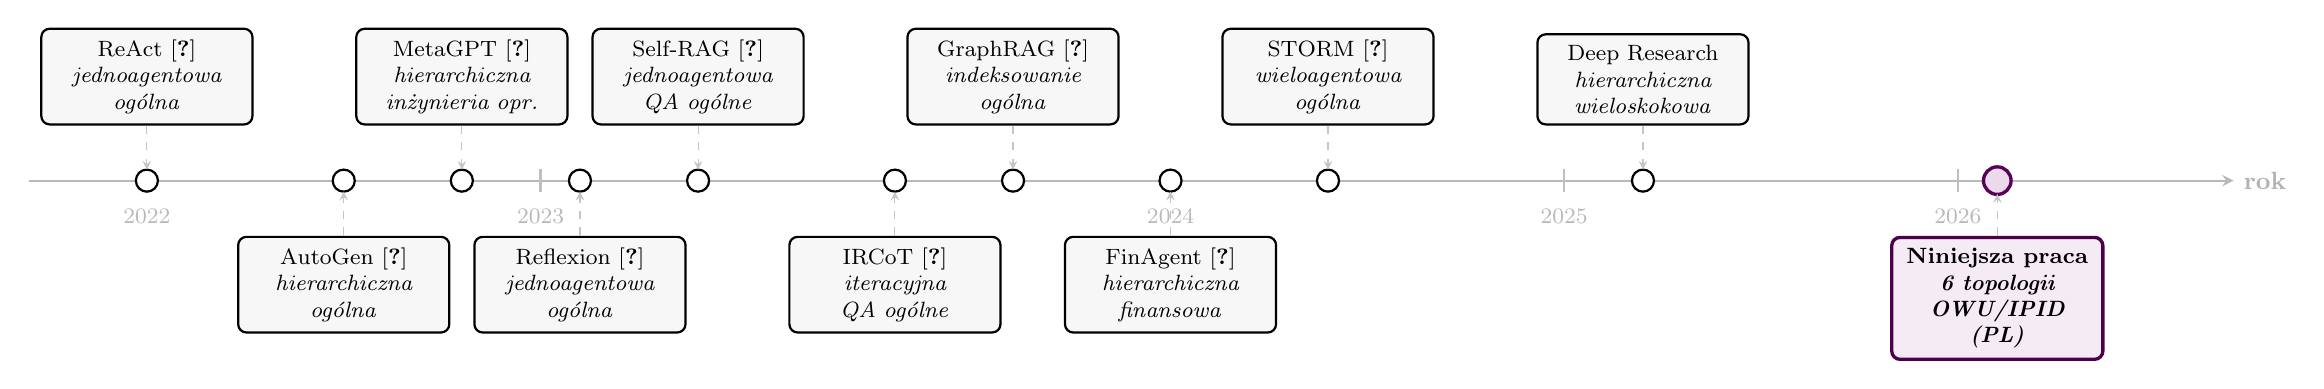
\begin{tikzpicture}[
        every node/.style={font=\small},
        dot/.style={circle, draw, thick, fill=white,
            minimum size=0.28cm, inner sep=0pt},
        dothighlight/.style={circle, draw=violet!70!black, very thick,
            fill=violet!15, minimum size=0.35cm, inner sep=0pt},
        workbox/.style={rectangle, draw, rounded corners=3pt, thick,
            text width=2.4cm, align=center, font=\footnotesize,
            fill=gray!6, inner sep=4pt},
        workboxhl/.style={rectangle, draw=violet!60!black, rounded corners=3pt,
            very thick, text width=2.4cm, align=center,
            font=\footnotesize\bfseries, fill=violet!8, inner sep=4pt},
        arrow/.style={->, >=stealth, thick, draw=gray!55},
        dasharrow/.style={->, >=stealth, dashed, thin, draw=gray!45}
      ]
      \draw[arrow] (-0.5, 0) -- (27.5, 0);
      \node[font=\small\bfseries, text=gray!60] at (27.9, 0) {rok};
      \foreach \x/\yr in {1.0/2022, 6.0/2023, 14.0/2024, 19.0/2025, 24.0/2026}{
          \draw[thick, gray!50] (\x, -0.15) -- (\x, 0.15);
          \node[font=\footnotesize, text=gray!55] at (\x, -0.45) {\yr};
        }
      \node[dot] at (1.0, 0) {};
      \node[workbox, above=0.7cm] (react) at (1.0, 0)
      {ReAct \cite{yao2022react}\\\textit{jednoagentowa\\ogólna}};
      \draw[dasharrow] (react.south) -- (1.0, 0.14);
      \node[dot] at (5.0, 0) {};
      \node[workbox, above=0.7cm] (metagpt) at (5.0, 0)
      {MetaGPT \cite{hong2023metagpt}\\\textit{hierarchiczna\\inżynieria opr.}};
      \draw[dasharrow] (metagpt.south) -- (5.0, 0.14);
      \node[dot] at (8.0, 0) {};
      \node[workbox, above=0.7cm] (selfrag) at (8.0, 0)
      {Self-RAG \cite{asai2023self}\\\textit{jednoagentowa\\QA ogólne}};
      \draw[dasharrow] (selfrag.south) -- (8.0, 0.14);
      \node[dot] at (3.5, 0) {};
      \node[workbox, below=0.7cm] (autogen) at (3.5, 0)
      {AutoGen \cite{wu2024autogen}\\\textit{hierarchiczna\\ogólna}};
      \draw[dasharrow] (autogen.north) -- (3.5, -0.14);
      \node[dot] at (6.5, 0) {};
      \node[workbox, below=0.7cm] (reflexion) at (6.5, 0)
      {Reflexion \cite{shinn2024reflexion}\\\textit{jednoagentowa\\ogólna}};
      \draw[dasharrow] (reflexion.north) -- (6.5, -0.14);
      \node[dot] at (12.0, 0) {};
      \node[workbox, above=0.7cm] (graphrag) at (12.0, 0)
      {GraphRAG \cite{edge2024local}\\\textit{indeksowanie\\ogólna}};
      \draw[dasharrow] (graphrag.south) -- (12.0, 0.14);
      \node[dot] at (16.0, 0) {};
      \node[workbox, above=0.7cm] (storm) at (16.0, 0)
      {STORM \cite{shao2024assisting}\\\textit{wieloagentowa\\ogólna}};
      \draw[dasharrow] (storm.south) -- (16.0, 0.14);
      \node[dot] at (14.0, 0) {};
      \node[workbox, below=0.7cm] (finagent) at (14.0, 0)
      {FinAgent \cite{zhang2024multimodal}\\\textit{hierarchiczna\\finansowa}};
      \draw[dasharrow] (finagent.north) -- (14.0, -0.14);
      \node[dot] at (10.5, 0) {};
      \node[workbox, below=0.7cm] (ircot) at (10.5, 0)
      {IRCoT \cite{trivedi2023interleaving}\\\textit{iteracyjna\\QA ogólne}};
      \draw[dasharrow] (ircot.north) -- (10.5, -0.14);
      \node[dot] at (20.0, 0) {};
      \node[workbox, above=0.7cm] (deepresearch) at (20.0, 0)
      {Deep Research\\\textit{hierarchiczna\\wieloskokowa}};
      \draw[dasharrow] (deepresearch.south) -- (20.0, 0.14);
      \node[dothighlight] at (24.5, 0) {};
      \node[workboxhl, below=0.7cm] (this) at (24.5, 0)
      {Niniejsza praca\\\textit{6 topologii\\OWU/IPID (PL)}};
      \draw[dasharrow] (this.north) -- (24.5, -0.17);
    \end{tikzpicture}
  \end{adjustbox}
  \zrodlo{opracowanie własne na podstawie literatury}
\end{figure}

\subsection{Luki badawcze i~wkład niniejszej pracy}\label{subsec:luki-badawcze-i-wklad-niniejszej-pracy}

Przegląd literatury ujawnia trzy wyraźne luki, które bezpośrednio motywują
projekt niniejszego badania. Żadna z~omówionych prac nie uwzględnia ich
wszystkich jednocześnie -- co oznacza, że mimo rozbudowanego dorobku w~obszarze
architektur agentowych i~systemów RAG, pytanie o~rzeczywisty wpływ topologii na
jakość odpowiedzi w~domenie regulacyjnej pozostaje otwarte.

Najistotniejszy jest brak kontrolowanych porównań wielu topologii przy stałym
modelu, tych samych narzędziach i~tym samym korpusie. W~każdej z~omówionych
prac trudno oddzielić wpływ topologii od wpływu lepszego wyszukiwania, bardziej
dopracowanych instrukcji systemowych lub innego modelu bazowego. Wang i~in.
oraz Xi i~in. wskazują ten brak jako jedną z~głównych przeszkód w~budowaniu
kumulatywnej wiedzy o~architekturach agentowych~\cite{wang2024survey,
  xi2025rise}. Nowa architektura zestawiana jest zazwyczaj z~prostym modelem
bazowym -- nie z~innymi architekturami w~identycznych warunkach -- co
uniemożliwia odpowiedź na pytanie, czy złożoność orkiestracji bezpośrednio
wpływa na wyższą jakość odpowiedzi, czy jedynie na wyższe koszty operacyjne.
Problem ten jest szczególnie widoczny, gdy wyniki poszczególnych prac są ze
sobą zestawiane: różnice w~modelu bazowym, zestawie narzędzi czy zbiorze
testowym sprawiają, że porównanie między architekturami opisywanymi w~różnych
publikacjach jest obarczone dużą niepewnością metodologiczną.

Drugą luką jest brak zestawu testowego dla dokumentów ubezpieczeniowych
w~języku polskim. Dostępne zbiory -- HotPotQA~\cite{yang2018hotpotqa},
Wikipedia, zadania programistyczne -- testują wnioskowanie wieloskokowe na
tekstach ogólnych i~nie obejmują problemów typowych dla tej domeny: sieci
wzajemnych odesłań między definicjami a~wyłączeniami, konieczności uzgadniania
sprzecznych postanowień czy porównywania zapisów z~wielu polis jednocześnie.
Polskojęzyczne zasoby ewaluacyjne dla tej dziedziny nie istnieją, co oznacza,
że wyniki uzyskane na zbiorach anglojęzycznych nie mogą być bezpośrednio
przeniesione na systemy operujące na polskich dokumentach regulacyjnych --
zarówno ze względu na różnice językowe, jak i~odmienną strukturę prawną.

Trzecia luka dotyczy głębokości analizy wyników. Dominujące podejście polega na
raportowaniu średnich wartości metryk jakościowych i~operacyjnych, co pozwala
co najwyżej uszeregować architektury według łącznego wyniku, lecz nie wyjaśnia
mechanizmów stojących za obserwowanymi różnicami. Wiedza o~tym, kiedy
i~dlaczego dany system zawodzi -- czy traci kontekst przy długich zadaniach,
czy błędnie klasyfikuje zapytania, czy propaguje błędy między modułami -- ma
bezpośrednią wartość przy wyborze architektury do zastosowania produkcyjnego.
Tymczasem analiza trybów niepowodzeń pozostaje w~literaturze nieobecna lub
ograniczona do kilku przykładów anegdotycznych.

Tabela~\ref{tab:zestawienie-prac-pokrewnych} zestawia omówione prace względem
tych trzech wymiarów. Każda ze zidentyfikowanych luk przekłada się bezpośrednio
na jeden z~wkładów badania: brak kontrolowanego porównania -- na projekt
eksperymentalny z~izolowaną topologią jako jedyną zmienną niezależną, przy
stałym modelu, narzędziach, korpusie i~zestawie 90~pytań dla wszystkich sześciu
architektur; brak polskiego zestawu testowego -- na oryginalny zestaw pytań
o~czterech poziomach trudności oparty wyłącznie na polskich dokumentach OWU
i~IPID, obejmujący zarówno pytania proste jak i~wymagające wieloetapowego
wnioskowania między sekcjami; brak analizy błędów -- na jakościowe badanie
śladów wykonania, które wykracza poza agregowane metryki i~pozwala
zidentyfikować wzorce niepowodzeń charakterystyczne dla każdej topologii wraz
z~rekomendacjami praktycznymi dla projektantów systemów produkcyjnych.

\begin{sidewaystable}[htbp]
  \caption{Zestawienie prac pokrewnych}\label{tab:zestawienie-prac-pokrewnych}
  \centering
  \small
  \renewcommand{\arraystretch}{1.3}
  \begin{tabularx}{0.95\textheight}{@{} p{2.8cm} p{2.8cm} p{3.5cm} p{3.5cm} p{3.5cm} X @{}}
    \toprule
    \textbf{System}
     & \textbf{Topologia}
     & \textbf{Dziedzina}
     & \textbf{Kontrolowane porównanie}
     & \textbf{Główna metryka}
     & \textbf{Luka względem niniejszej pracy}                                                        \\
    \midrule
    ReAct~\cite{yao2022react}
     & Jednoagentowa                                                      & Ogólna (Wikipedia)
     & Nie -- porównanie z~CoT                                            & Dokładność zadań
     & Brak domeny regulacyjnej, jedna topologia                                                      \\
    \addlinespace
    AutoGen~\cite{wu2024autogen}
     & Hierarchiczna, grupowa                                             & Kodowanie, ogólna
     & Nie -- brak wspólnego korpusu                                      & Wskaźnik sukcesu zadania
     & Brak kontrolowanego środowiska, brak QA na dokumentach                                         \\
    \addlinespace
    MetaGPT~\cite{hong2023metagpt}
     & Hierarchiczna                                                      & Inżynieria oprogramowania
     & Nie -- porównanie z~bazowym LLM                                    & Poprawność kodu
     & Brak domeny dokumentowej, jedna topologia                                                      \\
    \addlinespace
    FinAgent~\cite{zhang2024multimodal}
     & Hierarchiczna                                                      & Dokumenty finansowe
     & Nie -- brak linii bazowej jednoagentowej                           & Zwrot z~inwestycji
     & Brak kontrolowanego porównania topologii, domena finansowa                                     \\
    \addlinespace
    Self-RAG~\cite{asai2023self}
     & Jednoagentowa                                                      & Ogólna (QA)
     & Nie -- porównanie z~RAG                                            & Wierność, dokładność
     & Jedna topologia, brak domeny regulacyjnej                                                      \\
    \addlinespace
    Reflexion~\cite{shinn2024reflexion}
     & Jednoagentowa                                                      & Ogólna
     & Nie -- jedna architektura                                          & Wskaźnik sukcesu
     & Brak porównania topologii, brak dokumentów prawnych                                            \\
    \addlinespace
    GraphRAG~\cite{edge2024local}
     & Wzbogacone indeksowanie                                            & Ogólna (teksty długie)
     & Nie -- porównanie z~RAG                                            & Jakość odpowiedzi
     & Brak porównania topologii agentowych, brak domeny ubezpieczeniowej                             \\
    \addlinespace
    \rowcolor{violet!6}
    \textbf{Niniejsza praca}
     & \textbf{Sześć topologii}                                           & \textbf{Polskie OWU/IPID}
     & \textbf{Tak -- stały model, korpus, metryki}
     & \textbf{Wierność, poprawność, opóźnienie, tokeny}
     & \textbf{Kontrolowane porównanie, polska domena ubezpieczeniowa,
         analiza trybów niepowodzeń, rekomendacje produkcyjne}                                 \\
    \bottomrule
  \end{tabularx}
  \zrodlo{opracowanie własne na podstawie literatury}
\end{sidewaystable}
